\documentclass[11pt,a4paper]{article}
\usepackage[utf8]{inputenc}
\usepackage[italian]{babel}
\usepackage{geometry}
\usepackage{graphicx}
\usepackage{float}
\usepackage{tabularx}
\usepackage{booktabs}
\usepackage{hyperref}
\usepackage{fancyhdr}
\usepackage{lastpage}
\usepackage{longtable}

\geometry{margin=2.5cm}

% Intestazione e piè di pagina
\pagestyle{fancy}
\fancyhf{}
\renewcommand{\headrulewidth}{0pt}
\fancyfoot[C]{\thepage\ di \pageref{LastPage}}

\begin{document}

% Prima pagina - Intestazione
\begin{titlepage}
    \centering
    
    % Logo Università
    \begin{figure}[H]
        \centering
        
\includegraphics[width=0.3\textwidth]{../logoUnipd.jpg}
    \end{figure}
    
    \vspace{0.5cm}
    
    \textbf{\Large Università degli Studi di Padova} \\
    \vspace{0.2cm}
    \textbf{Laurea in Informatica} \\
    \vspace{0.2cm}
    \textbf{Corso di Ingegneria del Software} \\
    \vspace{0.2cm}
    \textbf{Anno Accademico 2025/2026} \\
    
    \vspace{1cm}
    
    % Logo gruppo
    \begin{figure}[H]
        \centering
        
\includegraphics[width=0.2\textwidth]{../LogoByteMe.jpg}
    \end{figure}
    
    \vspace{0.5cm}
    
    \textbf{\Large Gruppo ByteMe} \\
    \vspace{0.2cm}
    \texttt{byteme2025swe@gmail.com} \\
    
    \vspace{1cm}
    
    \textbf{\Huge Analisi dei Requisiti} \\
    
    \vspace{1.5cm}
    
    \begin{table}[H]
        \centering
        \begin{tabular}{|l|p{5cm}|}
            \hline
            \textbf{Versione} & 1.2.5 \\
            \hline
            \textbf{Stato} & In corso \\
            \hline
            \textbf{Redazione} & Tutto il gruppo \\
            \hline
            \textbf{Verifica} & Tutto il gruppo \\
            \hline
            \textbf{Approvazione} & Tutto il gruppo \\
            \hline
            \textbf{Proprietario} & ByteMe \\
            \hline
            \textbf{Uso} & Esterno \\
            \hline
            \textbf{Destinatari} & Prof. Tullio Vardanega \\ & Prof. Riccardo Cardin \\
            \hline
        \end{tabular}
    \end{table}
    
    \vfill
\end{titlepage}

% Seconda pagina - Versionamento
\thispagestyle{empty}
\section*{Registro dei Cambiamenti}

\begin{table}[H]
    \centering
    \begin{tabular}{|c|c|c|>{\raggedright\arraybackslash}p{0.4\textwidth}|c|}
        \hline
        \textbf{Versione} & \textbf{Data} & \textbf{Autore} & \textbf{Descrizione} & \textbf{Verifica} \\
        \hline
        1.2.5 & 01/01/2026 & Joseph Grant & Crosscheck requisiti relativi a macroarea 5, piccole correzioni e aggiunte &  \\
        \hline
        1.2.4 & 30/12/2025 & Giulia Barzon & Correzione requisiti macroarea 1 e inserimento diagrammi completi &  \\
        \hline
        1.2.3 & 29/12/2025 & Giulia Barzon & Aggiunti primi diagrammi casi d'uso &  Matteo Cuogo \\
        \hline
        1.2.2 & 29/12/2025 & Giulia Barzon & Rimosso vecchio caso d'uso 3.3 per incoerenza e sistemati relativi requisiti & Matteo Cuogo \\
        \hline
        1.2.1 & 29/12/2025 & Tommaso Tombacco & Modifiche ad alcuni casi d'uso &  \\ 
        \hline
        1.2.0 & 28/12/2025 & Joseph Grant & Aggiunta della maggioranza dei requisiti &  \\ 
        \hline
        1.1.5 & 27/12/2025 & Elisa Marchioro & Aggiunto sottocaso 4.3.1 & \\ 
        \hline
        1.1.4 & 27/12/2025 & Joseph Grant & Aggiunta sezione 'verifica' al versionamento & Elisa Marchioro\\ 
        \hline
        1.1.3 & 27/12/2025 & Matteo Cuogo & Correzione e ampliamento dei casi d'uso rivisti & Elisa Marchioro\\
        \hline
        1.1.2 & 14/12/2025 & Giulia Barzon & Correzione errori e scrittura introduzione e classificazione dei requisiti &\\
        \hline
        1.1.1 & 08/12/2025 & Giulia Barzon & Inserimento caso d'uso 1.9 (Unicode) e creazione primo diagramma caso d'uso di esempio (2.3 e 2.9-2.11) &\\
        \hline
        1.1.0 & 07/12/2025 & Giulia Barzon & Inserimeno casi d'uso identificati & \\
        \hline
        1.0.0 & 20/11/2025 & Giulia Barzon & Creazione del documento e scrittura introduzione & Elisa Marchioro\\
        \hline
    \end{tabular}
    \caption{Registro delle versioni del documento}
    \label{tab:versionamento}
\end{table}

\newpage

% Terza pagina - Indice
\tableofcontents
\thispagestyle{empty}
\newpage

% Dalla quarta pagina - Contenuto principale
\setcounter{page}{1}

\section{Introduzione}
\subsection{Scopo del documento}
Questo documento descrive l'analisi dei requisiti per il progetto \textbf{"Second Brain"}. Il documento definisce in modo dettagliato i casi d'uso e i requisiti del sistema, che combina un editor di testo Markdown con funzionalità AI avanzate per assistere gli utenti nella creazione, revisione e miglioramento dei contenuti testuali.

L'obiettivo principale è fornire una specifica completa delle funzionalità che il sistema deve implementare, classificando i requisiti in obbligatori, desiderabili e opzionali, in linea con le richieste della proponente Zucchetti.

\subsection{Glossario}
Per evitare ambiguità, i termini tecnici usati nel documento vengono definiti in modo più approfondito nel documento "Glossario" che si trova nella repository del gruppo nella cartella "Documenti\textunderscore interni".

I termini che vengono considerati meritevoli di approfondimenti sono indicati con una G a pedice.

\subsection{Riferimenti}
\subsubsection{Riferimenti normativi}
\begin{itemize}
    \item Norme di Progetto - Documento interno del gruppo ByteMe
    \item Regolamento del progetto didattico
\end{itemize}

\subsubsection{Riferimenti informativi}
\begin{itemize}
    \item Capitolato C6 "Second Brain", Zucchetti
    \item Slide del corso di Ingegneria del Software
    \item Verbali interni ed esterni
\end{itemize}

\newpage

\section{Descrizione del progetto}
\subsection{Obiettivi del prodotto}
Il progetto \textbf{Second Brain} si propone di rivoluzionare il processo di scrittura e organizzazione delle idee attraverso l'integrazione di Large Language Models\textsubscript{G} in un editor di testo moderno. Gli obiettivi principali sono:

\begin{itemize}
    \item Fornire uno strumento di \textit{note-taking} avanzato che combini la semplicità del Markdown\textsubscript{G} con la potenza dell'IA generativa.
    \item Implementare un sistema di \textit{critica intelligente} del testo basato sulla metodologia dei "Sei Cappelli per Pensare" di Edward De Bono.
    \item Semplificare il processo di scrittura attraverso funzionalità di correzione, rielaborazione, traduzione e ottimizzazione automatica del testo.
    \item Implementare un sistema di \textit{distant writing} che permette di generare un testo completo a partire da un breve prompt dell'utente.
\end{itemize}


\subsection{Funzionalità del prodotto}
Il sistema offre le seguenti funzionalità principali:

\begin{itemize}
    \item \textbf{Editor Markdown\textsubscript{G}} avanzato con anteprima in tempo reale
    \item \textbf{Integrazione LLM\textsubscript{G}} per operazioni su testo selezionato o completo
    \item \textbf{Comandi base di elaborazione}: riassunto, riscrittura, traduzione, correzione grammaticale
    \item \textbf{Sistema di critica testuale} basato sui 6 cappelli per pensare
    \item \textbf{Distant Writing\textsubscript{G}} per generazione guidata di contenuti
    \item \textbf{Persistenza dati} con salvataggio locale e opzionale su cloud
\end{itemize}

\subsection{Caratteristiche del prodotto}
Le caratteristiche distintive che rendono unico il prodotto sono:

\begin{itemize}
    \item \textbf{Architettura ibrida}: applicazione web con possibile estensione server-side
    \item \textbf{Interfaccia semplice}: design pulito per un editor chiaro e semplice e anteprima in tempo reale
    \item \textbf{Multi-piattaforma}: accessibile da qualsiasi browser moderno
    \item \textbf{Estensibilità}: architettura modulare che permette l'aggiunta di nuove funzionalità
    
\end{itemize}

\subsection{Utenti}
Il prodotto è rivolto alle seguenti categorie di utenti:

\begin{itemize}
    \item \textbf{Studenti}: per la stesura di appunti, riassunti e materiale di studio
    \item \textbf{Professionisti}: per la creazione di documenti aziendali, report e presentazioni
    \item \textbf{Scrittori e content creator}: per l'ideazione, stesura e revisione di contenuti
    \item \textbf{Ricercatori}: per l'organizzazione di appunti di ricerca e letteratura
    \item \textbf{Utenti generici}: chiunque abbia bisogno di un editor per esigenze di scrittura assistita
\end{itemize}

Non sono richieste competenze tecniche avanzate per l'utilizzo delle funzionalità base, rendendo il prodotto accessibile a un'ampia gamma di utenti.

\newpage

\section{Casi d'uso}
\subsection{Introduzione}
Questa sezione descrive in dettaglio i casi d'uso del sistema \textbf{Second Brain}, identificando tutte le interazioni significative tra gli attori e il sistema. Il gruppo ha deciso di suddividere i casi d'uso in macroaree per organizzare in modo più chiaro i casi d'uso individuati. Ogni caso d'uso è definito attraverso:

\begin{itemize}
    \item \textbf{Codice identificativo} univoco seguendo lo schema UC-X.Y
    \item \textbf{Descrizione} chiara e concisa dello scenario
    \item \textbf{Attori} coinvolti nell'interazione
    \item \textbf{Precondizioni} necessarie per l'esecuzione
    \item \textbf{Postcondizioni} risultanti dall'esecuzione
    \item \textbf{Scenario principale} con sequenza di passi
\end{itemize}

I casi d'uso sono organizzati per macroaree funzionali per facilitare la lettura e il tracciamento.

\subsection{Attori}
Il sistema prevede i seguenti attori:

\begin{itemize}
    \item \textbf{Utente Non Autenticato\textsubscript{G}}: utente che accede alle funzionalità base senza registrazione
    \item \textbf{Utente Autenticato\textsubscript{G}}: utente registrato che accede alle funzionalità avanzate e alla persistenza cloud
    \item \textbf{Sistema AI\textsubscript{G}}: componente di intelligenza artificiale che elabora le richieste testuali
    \item \textbf{Sistema di Persistenza\textsubscript{G}}: componente responsabile del salvataggio e recupero dei dati
\end{itemize}

L'attore principale è l'\textbf{Utente} (nelle sue due varianti), mentre gli altri attori sono considerati secondari e interagiscono con il sistema in modo trasparente all'utente finale.

\newpage

\subsection{Macroarea 1 - Editor di testo}
\subsubsection{UC-1.0 - Utilizzo base dell'editor di testo}
\begin{itemize}
    \item \textbf{Attore principale}: Utente generico
    \item \textbf{Descrizione}: Utilizzo delle funzionalità base dell'editor di testo Markdown
    \item \textbf{Precondizioni}: L'utente è connesso a Internet e l'applicazione è pronta all'uso
    \item \textbf{Postcondizioni}: Il testo è stato inserito nell'editor e il documento è formattato rispettando la scrittura in Markdown
    \item \textbf{Scenario principale}:
        \begin{itemize}
            \item L'utente si connette ed entra nel sito
            \item L'utente inserisce testo semplice nell'area di editing
            \item L'utente utilizza la tastiera per digitare e modificare il testo
            \item Il sistema registra le modifiche in tempo reale
        \end{itemize}
    \item \textbf{Estensioni}:
        \begin{itemize}
            \item La connessione Internet viene persa durante la digitazione:
                \begin{enumerate}
                    \item Il sistema salva localmente le modifiche (opzionale)
                    \item Sincronizza quando la connessione ritorna disponibile
                \end{enumerate}
            \item L'editor non risponde ai comandi:
                \begin{enumerate}
                    \item Il sistema mostra un messaggio di errore
                    \item Suggerisce di ricaricare la pagina
                \end{enumerate}
        \end{itemize}
\end{itemize}

\subsubsection{UC-1.1 - Visualizzazione anteprima in tempo reale}
\begin{itemize}
    \item \textbf{Attore principale}: Utente generico
    \item \textbf{Descrizione}: Visualizzazione in tempo reale del testo formattato
    \item \textbf{Precondizioni}: L'editor contiene testo con sintassi Markdown
    \item \textbf{Postcondizioni}: Viene visualizzata l'anteprima formattata del testo in un'area apposita
    \item \textbf{Scenario principale}:
        \begin{itemize}
            \item L'utente modifica il testo nell'editor
            \item L’utente preme il pulsante “Compila”
            \item Il sistema elabora la sintassi Markdown
            \item Il sistema aggiorna il pannello di preview mostrando l’anteprima formattata del documento
            \item L'utente può confrontare editing e risultato finale
        \end{itemize}
    \item \textbf{Estensioni}:
        \begin{itemize}
            \item L'anteprima non si aggiorna correttamente:
                \begin{enumerate}
                    \item Il sistema forza un refresh manuale o segnala errore
                \end{enumerate}
            \item Il testo Markdown contiene errori di sintassi:
                \begin{enumerate}
                    \item L'anteprima mostra il testo non formattato o segnala errore
                \end{enumerate}
        \end{itemize}
\end{itemize}

\subsubsection{UC-1.2 - Selezione e modifica testo}
\begin{itemize}
    \item \textbf{Attore principale}: Utente generico
    \item \textbf{Descrizione}: Selezione e modifica di porzioni di testo nell'editor
    \item \textbf{Precondizioni}: È presente testo nell'editor
    \item \textbf{Postcondizioni}: Una porzione di testo viene selezionata e/o modificata
    \item \textbf{Scenario principale}:
        \begin{itemize}
            \item L'utente evidenzia una porzione di testo con il mouse o tastiera
            \item L'utente esegue operazioni di modifica (copia, taglia, incolla, cancella)
            \item Il sistema applica le modifiche alla selezione
        \end{itemize}
    \item \textbf{Estensioni}:
        \begin{itemize}
            \item La selezione include parti di sintassi Markdown:
                \begin{enumerate}
                    \item Il sistema gestisce la selezione preservando la formattazione
                \end{enumerate}
        \end{itemize}
\end{itemize}

% DIAGRAMMA
\begin{figure}[H]
    \centering
    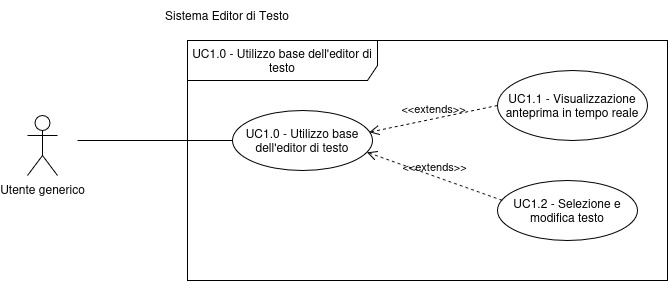
\includegraphics[width=0.8\textwidth]{../UCimg/UC1.0_utilizzoBaseEditor.jpg}
    \caption{Diagramma dei casi d'uso UC-1.0, 1.1, 1.2}
    \label{fig:uc1.0}
\end{figure}

\subsubsection{UC-1.3 - Copiare il testo}
\begin{itemize}
    \item \textbf{Attore principale}: Utente generico
    \item \textbf{Descrizione}: L'utente copia una parte di testo dall'area di modifica testo
    \item \textbf{Precondizioni}: Testo presente e selezionato
    \item \textbf{Postcondizioni}: L'utente ha copiato il testo da lui selezionato
    \item \textbf{Scenario principale}:
        \begin{itemize}
            \item L'utente seleziona una porzione di testo
            \item L'utente utilizza il comando "Copia" tramite:
                \begin{enumerate}
                    \item Tasto di scelta rapida (Ctrl+C)
                    \item Menu contestuale (tasto destro)
                    \item Toolbar dell'editor (opzionale)
                \end{enumerate}
            \item Il testo selezionato viene copiato negli appunti di sistema
        \end{itemize}
\end{itemize}

% DIAGRAMMA
\begin{figure}[H]
    \centering
    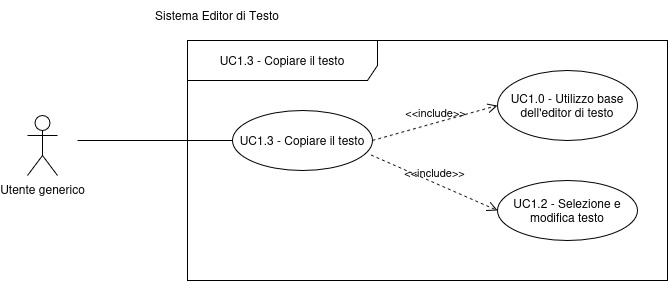
\includegraphics[width=0.8\textwidth]{../UCimg/UC1.3_copia.jpg}
    \caption{Diagramma del caso d'uso UC-1.3}
    \label{fig:uc1.3}
\end{figure}

\subsubsection{UC-1.4 - Incollare il testo}
\begin{itemize}
    \item \textbf{Attore principale}: Utente generico
    \item \textbf{Descrizione}: L'utente incolla una parte di testo nell'area di modifica testo
    \item \textbf{Precondizioni}: Testo presente negli appunti di sistema
    \item \textbf{Postcondizioni}: L'utente ha incollato il testo precedentemente copiato
    \item \textbf{Scenario principale}:
        \begin{itemize}
            \item L'utente posiziona il cursore nel punto desiderato
            \item L'utente utilizza il comando "Incolla" tramite:
                \begin{enumerate}
                    \item Tasto di scelta rapida (Ctrl+V)
                    \item Menu contestuale (tasto destro)
                    \item Toolbar dell'editor (opzionale)
                \end{enumerate}
            \item Il testo dagli appunti viene inserito nella posizione del cursore
        \end{itemize}
\end{itemize}
\begin{figure}[H]
    \centering
    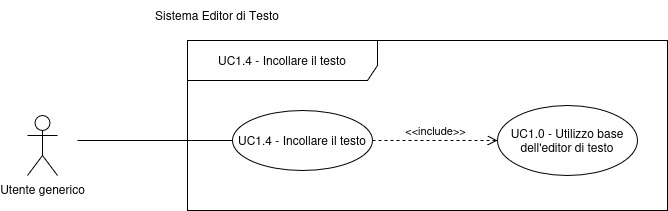
\includegraphics[width=0.8\textwidth]{../UCimg/UC1.4_incolla.jpg}
    \caption{Diagramma del caso d'uso UC-1.4}
    \label{fig:uc1.4}
\end{figure}

\subsubsection{UC-1.5 - Tagliare il testo}
\begin{itemize}
    \item \textbf{Attore principale}: Utente generico
    \item \textbf{Descrizione}: L'utente taglia una parte di testo dall'area di modifica, rimuovendola dal documento e copiandola negli appunti
    \item \textbf{Precondizioni}: Testo presente e selezionato
    \item \textbf{Postcondizioni}: Il testo selezionato viene rimosso dall'editor e salvato negli appunti di sistema
    \item \textbf{Scenario principale}:
        \begin{itemize}
            \item L'utente seleziona una porzione di testo
            \item L'utente utilizza il comando "Taglia" tramite:
                \begin{enumerate}
                    \item Tasto di scelta rapida (Ctrl+X)
                    \item Menu contestuale (tasto destro)
                    \item Toolbar dell'editor (opzionale)
                \end{enumerate}
            \item Il sistema rimuove il testo selezionato dall'editor
            \item Il testo rimosso viene salvato negli appunti di sistema
        \end{itemize}
\end{itemize}
\begin{figure}[H]
    \centering
    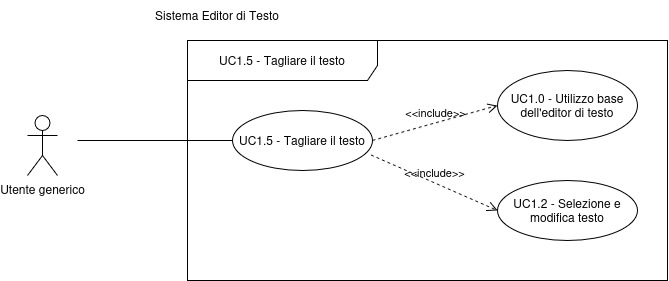
\includegraphics[width=0.8\textwidth]{../UCimg/UC1.5_taglia.jpg}
    \caption{Diagramma del caso d'uso UC-1.5}
    \label{fig:uc1.5}
\end{figure}

\subsubsection{UC-1.6 - Annullamento modifica (Undo)}
\begin{itemize}
    \item \textbf{Attore principale}: Utente generico
    \item \textbf{Descrizione}: Annullamento dell'ultima operazione di modifica effettuata
    \item \textbf{Precondizioni}: È stata effettuata almeno una modifica al testo e l'utente desidera annullare l'ultima operazione eseguita
    \item \textbf{Postcondizioni}: Il testo ritorna allo stato precedente l'ultima modifica
    \item \textbf{Scenario principale}:
        \begin{itemize}
            \item L'utente effettua una modifica al testo che non soddisfa le sue aspettative
            \item L'utente seleziona l'opzione "Annulla" tramite:
                \begin{enumerate}
                    \item Tasto di scelta rapida (Ctrl+Z)
                    \item Pulsante nella toolbar dell'editor (freccia verso sinistra)
                \end{enumerate}
            \item Il sistema ripristina il testo allo stato precedente la modifica
            \item L'operazione annullata viene spostata nella coda redo
        \end{itemize}
    \item \textbf{Estensioni}:
        \begin{itemize}
            \item Non ci sono operazioni da annullare:
                \begin{enumerate}
                    \item Il comando undo è disabilitato
                \end{enumerate}
        \end{itemize}
\end{itemize}

\subsubsection{UC-1.7 - Ripristino modifica (Redo)}
\begin{itemize}
    \item \textbf{Attore principale}: Utente generico
    \item \textbf{Descrizione}: Ripristino di un'operazione precedentemente annullata
    \item \textbf{Precondizioni}: È stata effettuata almeno un'operazione di undo; l'utente desidera ripristinare un'operazione precedentemente annullata
    \item \textbf{Postcondizioni}: Il testo ritorna allo stato successivo all'operazione ripristinata
    \item \textbf{Scenario principale}:
        \begin{itemize}
            \item L'utente ha annullato una o più operazioni con undo
            \item L'utente decide di ripristinare un'operazione annullata
            \item L'utente seleziona l'opzione "Ripristina" tramite:
                \begin{enumerate}
                    \item Tasto di scelta rapida (Ctrl+Y o Ctrl+Shift+Z)
                    \item Pulsante nella toolbar dell'editor
                \end{enumerate}
            \item Il sistema riapplica l'ultima operazione annullata
            \item L'operazione viene rimossa dalla coda redo
        \end{itemize}
    \item \textbf{Estensioni}:
        \begin{itemize}
            \item Non ci sono operazioni da ripristinare:
                \begin{enumerate}
                    \item Il comando redo è disabilitato
                \end{enumerate}
        \end{itemize}
\end{itemize}
\begin{figure}[H]
    \centering
    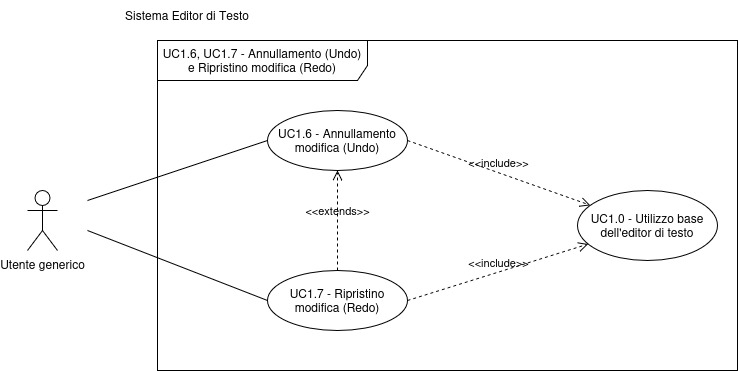
\includegraphics[width=0.8\textwidth]{../UCimg/UC1.6_1.7_undo_redo.jpg}
    \caption{Diagramma dei casi d'uso UC-1.6 e UC-1.7}
    \label{fig:uc1.6}
\end{figure}

\subsubsection{UC-1.8 - Modifica del testo tramite barra degli strumenti}
\begin{itemize}
    \item \textbf{Attore principale}: Utente generico
    \item \textbf{Descrizione}: Formattazione del testo tramite la barra degli strumenti dell'editor
    \item \textbf{Precondizioni}: È presente testo nell'editor pronto per essere modificato
    \item \textbf{Postcondizioni}: Il testo selezionato viene formattato secondo la sintassi Markdown
    \item \textbf{Scenario principale}:
        \begin{itemize}
            \item L'utente seleziona il testo da formattare
            \item L'utente clicca sul pulsante desiderato nella barra degli strumenti
            \item Il sistema applica automaticamente la sintassi Markdown corrispondente
            \item Il testo viene visualizzato formattato nell'anteprima
        \end{itemize}
    \item \textbf{Estensioni}:
        \begin{itemize}
            \item Combinazione di più formattazioni diverse:
                \begin{enumerate}
                    \item Il sistema gestisce le formattazioni multiple mettendole insieme
                \end{enumerate}
            \item Il testo ha già una specifica formattazione e l'utente la applica di nuovo:
                \begin{enumerate}
                    \item Il sistema rimuove la formattazione
                \end{enumerate}
            \item Selezione di testo che è parzialmente formattato:
                \begin{enumerate}
                    \item Tutto il testo viene formattato
                \end{enumerate}
        \end{itemize}
\end{itemize}

\subsubsection{UC-1.8.1 - Applicazione grassetto al testo}
\begin{itemize}
    \item \textbf{Attore principale}: Utente generico
    \item \textbf{Descrizione}: Formattazione del testo in grassetto tramite barra degli strumenti
    \item \textbf{Precondizioni}: È presente testo selezionato nell'editor
    \item \textbf{Postcondizioni}: Il testo selezionato viene formattato in grassetto
    \item \textbf{Scenario principale}:
        \begin{itemize}
            \item L'utente seleziona il testo da rendere in grassetto
            \item L'utente clicca sul pulsante "Grassetto" nella toolbar
            \item Il sistema applica la sintassi Markdown per il grassetto
            \item Il testo viene visualizzato in grassetto nell'anteprima
        \end{itemize}
    \item \textbf{Estensioni}:
        \begin{itemize}
            \item Il testo è già in grassetto:
                \begin{enumerate}
                    \item Il sistema rimuove la formattazione
                \end{enumerate}
            \item Selezione di testo che è parzialmente in grassetto:
                \begin{enumerate}
                    \item Tutto il testo viene formattato in grassetto
                \end{enumerate}
        \end{itemize}
\end{itemize}

\subsubsection{UC-1.8.2 - Applicazione corsivo al testo}
\begin{itemize}
    \item \textbf{Attore principale}: Utente generico
    \item \textbf{Descrizione}: Formattazione del testo in corsivo tramite barra degli strumenti
    \item \textbf{Precondizioni}: È presente testo selezionato nell'editor
    \item \textbf{Postcondizioni}: Il testo selezionato viene formattato in corsivo
    \item \textbf{Scenario principale}:
        \begin{itemize}
            \item L'utente seleziona il testo da rendere in corsivo
            \item L'utente clicca sul pulsante "Corsivo" nella toolbar
            \item Il sistema applica la sintassi Markdown per il corsivo
            \item Il testo viene visualizzato in corsivo nell'anteprima
        \end{itemize}
\end{itemize}

\subsubsection{UC-1.8.3 - Applicazione sottolineato al testo}
\begin{itemize}
    \item \textbf{Attore principale}: Utente generico
    \item \textbf{Descrizione}: Formattazione del testo come sottolineato tramite barra degli strumenti
    \item \textbf{Precondizioni}: È presente testo selezionato nell'editor
    \item \textbf{Postcondizioni}: Il testo selezionato viene formattato come sottolineato
    \item \textbf{Scenario principale}:
        \begin{itemize}
            \item L'utente seleziona il testo da rendere sottolineato
            \item L'utente clicca sul pulsante "Sottolineato" nella toolbar
            \item Il sistema applica la sintassi Markdown per sottolineare il testo
            \item Il testo viene visualizzato sottolineato nell'anteprima
        \end{itemize}
\end{itemize}

\subsubsection{UC-1.8.4 - Gestione intestazioni e struttura documento}
\begin{itemize}
    \item \textbf{Attore principale}: Utente generico
    \item \textbf{Descrizione}: Applicazione di intestazioni e struttura al documento
    \item \textbf{Precondizioni}: L'editor è aperto e pronto per la scrittura
    \item \textbf{Postcondizioni}: Vengono applicate intestazioni e struttura al documento
    \item \textbf{Scenario principale}:
        \begin{itemize}
            \item L'utente posiziona il cursore dove inserire l'intestazione
            \item L'utente applica un'intestazione tramite:
                \begin{enumerate}
                    \item Toolbar (H1, H2, H3, ecc.)
                    \item Sintassi Markdown (\#, \#\#, \#\#\#)
                    \item Tasti di scelta rapida
                \end{enumerate}
            \item Il sistema formatta il testo come intestazione
        \end{itemize}
\end{itemize}

\subsubsection{UC-1.8.5 - Inserimento liste ed elenchi}
\begin{itemize}
    \item \textbf{Attore principale}: Utente generico
    \item \textbf{Descrizione}: Creazione di liste ordinate e non ordinate nel documento
    \item \textbf{Precondizioni}: L'editor è aperto e pronto per la scrittura
    \item \textbf{Postcondizioni}: Viene creata una lista ordinata o non ordinata
    \item \textbf{Scenario principale}:
        \begin{itemize}
            \item L'utente posiziona il cursore dove inserire la lista
            \item L'utente seleziona il tipo di lista (ordinata/non ordinata)
            \item L'utente inserisce gli elementi della lista
            \item Il sistema formatta automaticamente la lista
        \end{itemize}
    \item \textbf{Estensioni}:
        \begin{itemize}
            \item Inserimento di sotto-liste:
                \begin{enumerate}
                    \item Il sistema gestisce l'indentazione automatica
                \end{enumerate}
            \item Numerazione automatica per liste ordinate:
                \begin{enumerate}
                    \item Il sistema mantiene la numerazione corretta
                \end{enumerate}
        \end{itemize}
\end{itemize}

\subsubsection{UC-1.8.6 - Inserimento link e riferimenti}
\begin{itemize}
    \item \textbf{Attore principale}: Utente generico
    \item \textbf{Descrizione}: Inserimento di link ipertestuali nel documento
    \item \textbf{Precondizioni}: È presente testo da collegare o l'utente vuole inserire un link
    \item \textbf{Postcondizioni}: Viene inserito un link ipertestuale nel documento
    \item \textbf{Scenario principale}:
        \begin{itemize}
            \item L'utente seleziona il testo da trasformare in link
            \item L'utente clicca sul comando "Inserisci link"
            \item L'utente inserisce l'URL di destinazione
            \item Il sistema applica la sintassi Markdown per il link
        \end{itemize}
\end{itemize}
\begin{figure}[H]
    \centering
    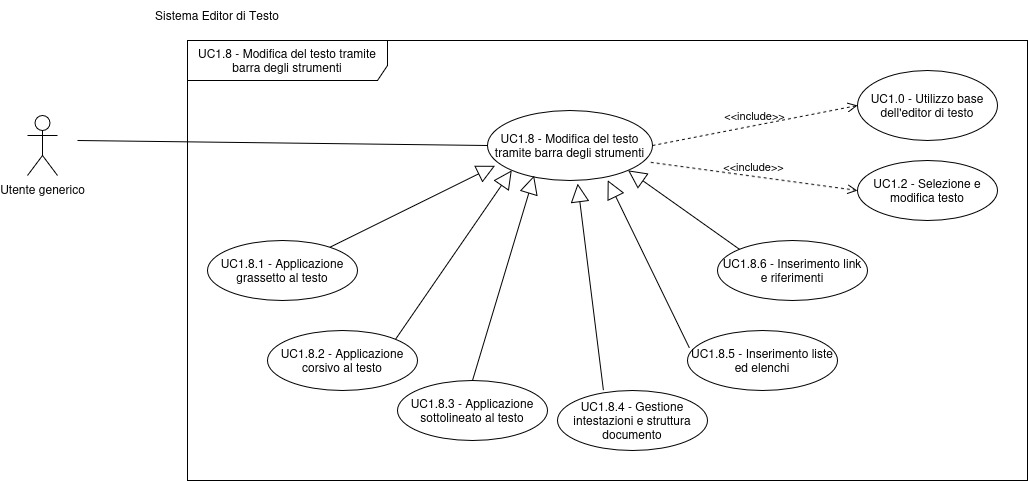
\includegraphics[width=0.8\textwidth]{../UCimg/UC1.8_toolbar.jpg}
    \caption{Diagramma dei casi d'uso UC-1.8 e UC-1.8.*}
    \label{fig:uc1.8}
\end{figure}

\subsubsection{UC-1.9 - Modalità di visualizzazione editor}
\begin{itemize}
    \item \textbf{Attore principale}: Utente generico
    \item \textbf{Descrizione}: Cambio della modalità di visualizzazione dell'editor
    \item \textbf{Precondizioni}: L'editor contiene testo
    \item \textbf{Postcondizioni}: Cambia la modalità di visualizzazione dell'editor
    \item \textbf{Scenario principale}:
        \begin{itemize}
            \item L'utente seleziona una modalità di visualizzazione:
                \begin{enumerate}
                    \item Solo editor (sintassi Markdown visibile)
                    \item Solo anteprima (risultato formattato)
                    \item Split view (editor e anteprima affiancati)
                \end{enumerate}
            \item Il sistema adatta l'interfaccia alla modalità scelta
        \end{itemize}
    \item \textbf{Estensioni}:
        \begin{itemize}
            \item Ridimensionamento della finestra in split view:
                \begin{enumerate}
                    \item Il sistema adatta dinamicamente le dimensioni
                \end{enumerate}
        \end{itemize}
\end{itemize}

\subsubsection{UC-1.10 - Supporto caratteri multilingua (Unicode)}
\begin{itemize}
    \item \textbf{Attore principale}: Utente generico
    \item \textbf{Descrizione}: L'editor supporta l'inserimento, visualizzazione e modifica di caratteri Unicode, permettendo la scrittura in lingue diverse dall'italiano/inglese e garantendo la corretta formattazione Markdown anche con tali caratteri.
    \item \textbf{Precondizioni}: L'editor è aperto e l'utente ha configurato il proprio sistema per scrivere in una lingua supportata
    \item \textbf{Postcondizioni}: Il testo in qualsiasi lingua supportata può essere scritto, formattato e processato dall'AI
    \item \textbf{Scenario principale}:
        \begin{itemize}
            \item L'utente seleziona una lingua di input se utilizza caratteri non latini
            \item L'utente digita testo contenente tali caratteri direttamente nell'editor
            \item L'editor visualizza correttamente i caratteri Unicode e l'utente può applicare formattazione Markdown normalmente
            \item L'anteprima in tempo reale mostra la formattazione applicata correttamente
            \item L'utente può utilizzare le funzionalità AI (es. traduzione, correzione) sul testo Unicode senza errori
        \end{itemize}
    \item \textbf{Estensioni}:
        \begin{itemize}
            \item Se il browser o il sistema non supportano un determinato set di caratteri:
                \begin{enumerate}
                    \item L'editor visualizza placeholder (es. quadratini) e notifica all'utente il problema
                \end{enumerate}
            \item Se un font non supporta determinati caratteri:
                \begin{enumerate}
                    \item L'editor usa automaticamente un font di fallback
                    \item Mostra un avviso suggerendo di installare font appropriati
                \end{enumerate}
            \item Problemi con input method per lingue asiatiche (supporto per input method editor):
                \begin{enumerate}
                    \item L'editor mantiene la compatibilità con IME standard
                    \item Supporta composizione di caratteri complessi
                \end{enumerate}
        \end{itemize}
\end{itemize}


\subsubsection{UC-1.11 - Ricerca nel testo (opzionale)}
\begin{itemize}
    \item \textbf{Attore principale}: Utente generico
    \item \textbf{Descrizione}: Ricerca di occorrenze di testo all'interno del documento
    \item \textbf{Precondizioni}: È presente testo nell'editor
    \item \textbf{Postcondizioni}: Vengono trovate occorrenze di testo
    \item \textbf{Scenario principale}:
        \begin{itemize}
            \item L'utente attiva la funzione "Ricerca"
            \item L'utente inserisce il testo da cercare
            \item Il sistema evidenzia le occorrenze trovate
        \end{itemize}
    \item \textbf{Estensioni}:
        \begin{itemize}
            \item Nessuna occorrenza trovata:
                \begin{enumerate}
                    \item Il sistema informa l'utente
                \end{enumerate}
        \end{itemize}
\end{itemize}


\newpage

\subsection{Macroarea 2 - Funzionalità AI}
\subsubsection{UC-2.0 - Selezione testo per operazioni AI}
\begin{itemize}
    \item \textbf{Attore principale}: Utente generico
    \item \textbf{Descrizione}: Permette all’utente di selezionare una porzione di testo nell’editor per applicare operazioni di AI
    \item \textbf{Precondizioni}: È presente testo nell'editor
    \item \textbf{Postcondizioni}: Una porzione di testo viene selezionata per operazioni AI
    \item \textbf{Scenario principale}: 
        \begin{itemize}
            \item L'utente evidenzia una porzione di testo nell'editor
            \item È presente un menù con le opzioni AI disponibili
            \item L'utente seleziona l'operazione desiderata
            \item Il sistema applica l'operazione solo al testo selezionato
        \end{itemize}
    \item \textbf{Estensioni}: 
         \begin{enumerate}
            \item L'utente non seleziona alcun testo prima di scegliere un'operazione AI:
                \begin{itemize}
                    \item L'operazione AI viene applicata a tutto il testo presente nell'editor
                \end{itemize}
        \end{enumerate}
\end{itemize}

\subsubsection{UC-2.1 - Mantenimento e Interazione con i testi Generati dall'AI}
\begin{itemize}
    \item \textbf{Attore principale}: Utente generico
    \item \textbf{Descrizione}: Gestione della storia e interazione con tutti i testi generati dall’AI all’interno
del documento
    \item \textbf{Precondizioni}: Sono state eseguite una o più operazioni AI e i relativi testi generati sono stati inseriti nell'editor
    \item \textbf{Postcondizioni}: L'utente può visualizzare e operare sull'intera sequenza di generazioni AI accumulate nel documento
    \item \textbf{Scenario principale}:
        \begin{itemize}
            \item L'utente seleziona un'operazione AI da eseguire nel testo selezionato o non selezionato
            \item Ogni nuova operazione AI genera testo che viene inserito nell'editor sotto alla porzione di testo interessata o in un box apposito
            \item Le generazioni si accumulano come blocchi di testo distinti nel flusso del documento
            \item Ogni blocco mantiene la sua formattazione distintiva che identifica:
                \begin{enumerate}
                    \item Il tipo di operazione
                    \item La data/ora di generazione
                    \item I parametri specifici (lingua, cappello, ecc.)
                \end{enumerate}
            \item Il documento stesso diventa la cronologia visibile delle operazioni AI
            \item Visualizzazione contestuale della storia:
                \begin{enumerate}
                    \item L'utente scorre il documento e vede tutte le generazioni AI in sequenza
                    \item Le generazioni sono intercalate con il testo utente originale
                    \item La posizione relativa nel documento preserva il contesto temporale e logico
                \end{enumerate}
            \item L'utente può effettuare operazioni sulle generazioni:
                \begin{enumerate}
                    \item Modifica qualsiasi del testo generato
                    \item Eliminazione di singole generazioni
                    \item Ordinamento delle generazioni spostandole nel documento
                    \item Raggruppamento di generazioni correlate (es: tutte le traduzioni di un paragrafo)
                    \item Nascondere/mostrare intere sezioni di generazioni
                \end{enumerate}
        \end{itemize}
    \item \textbf{Estensioni}:
        \begin{itemize}
            \item L'utente vuole una vista compatta della storia:
                \begin{enumerate}
                    \item Opzione "Mostra solo testo utente" nasconde temporaneamente tutte le generazioni
                    \item Opzione "Mostra solo generazioni AI" evidenzia solo i blocchi generati
                \end{enumerate}
        \end{itemize}
\end{itemize}

\subsubsection{UC-2.2 - Distinzione del Testo Utente da quello Generato}
\begin{itemize}
    \item \textbf{Attore principale}: Utente generico
    \item \textbf{Descrizione}: Sistema di formattazione che rende chiaramente distinguibile il testo generato dall'AI dal testo scritto dall'utente
    \item \textbf{Precondizioni}: Nell'editor è presente sia testo digitato dall'utente che testo generato dal sistema
    \item \textbf{Postcondizioni}: Il testo generato è chiaramente distinguibile dal testo dell'utente
    \item \textbf{Scenario principale}:
        \begin{itemize}
            \item Il sistema formatta automaticamente il testo generato con:
                \begin{enumerate}
                    \item Una riga separatrice orizzontale (---) o altro elemento separatore
                    \item Commento iniziale in corsivo e grigio: Generato da AI - [tipo operazione] - [data]
                    \item Sfondo colorato leggero (es. azzurro chiaro per traduzioni, verde chiaro per riassunti) (opzionale)
                    \item un’area apposita (box) identificativa
                    \item colore del testo generato diverso dal colore del testo dell’utente (opzionale)
                \end{enumerate}
            \item L'utente può modificare il testo generato dall’AI tramite i comandi per accettare, eliminare o rigenerare la risposta, presenti nell’area identificativa
            \item L’utente può modificare sia il testo originale sia il testo generato dall’AI
        \end{itemize}
    \item \textbf{Estensioni}:
        \begin{itemize}
            \item L'utente modifica il testo generato dall'AI:
                \begin{enumerate}
                    \item Il sistema elimina automaticamente gli elementi distintivi dell’area identificativa del testo generato (opzionale)
                    \item Il testo assume lo stile standard dell’editor
                \end{enumerate}
        \end{itemize}
\end{itemize}

\subsubsection{UC-2.3 - Riassunto del testo}
\begin{itemize}
    \item \textbf{Attore principale}: Utente generico
    \item \textbf{Descrizione}: Generazione di un riassunto del testo selezionato o dell'intero documento
    \item \textbf{Precondizioni}: È presente testo nell'editor (completo o selezionato)
    \item \textbf{Postcondizioni}: Viene generato un riassunto del testo nell'editor con formattazione distintiva rispetto al testo originale
    \item \textbf{Scenario principale}:
        \begin{itemize}
            \item L'utente seleziona il testo da riassumere (opzionale)
            \item L'utente clicca sul comando "Riassumi"
            \item Il sistema invia il testo al LLM
            \item Il sistema mostra il riassunto generato sotto il testo originale, distinguendolo con elementi predefiniti
            \item L'utente può scegliere di mantenere o modificare sia il testo originale sia il testo generato
        \end{itemize}
    \item \textbf{Estensioni}:
        \begin{itemize}
            \item L'utente annulla l'operazione prima del completamento:
                \begin{enumerate}
                    \item Il testo originale rimane invariato
                \end{enumerate}
            \item LLM dà errore:
                \begin{enumerate}
                    \item Il sistema notifica l'errore all'utente
                    \item L'operazione viene annullata
                \end{enumerate}
        \end{itemize}
\end{itemize}

% DIAGRAMMA
\begin{figure}[H]
    \centering
    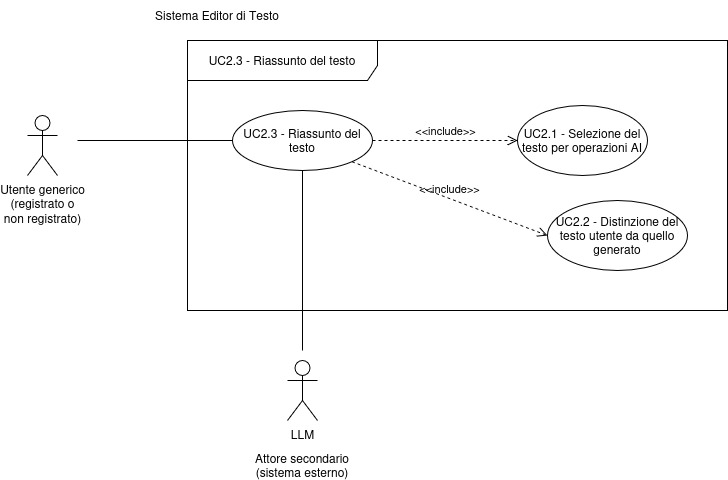
\includegraphics[width=0.8\textwidth]{../UCimg/UC2.3_riassunto.jpg}
    \caption{Diagramma del caso d'uso UC-2.3}
    \label{fig:uc2.3}
\end{figure}

\subsubsection{UC-2.4 - Riscrittura del testo}
\begin{itemize}
    \item \textbf{Attore principale}: Utente generico
    \item \textbf{Descrizione}: Rielaborazione del testo per migliorarne stile, sintassi e chiarezza
    \item \textbf{Precondizioni}: È presente testo nell'editor (completo o selezionato)
    \item \textbf{Postcondizioni}: Il testo viene riscritto secondo le specifiche dell'utente nell’editor con formattazione distintiva rispetto al testo originale
    \item \textbf{Scenario principale}:
        \begin{itemize}
            \item L'utente seleziona il testo da riscrivere
            \item L'utente clicca sul comando "Riscrivi"
            \item L'utente specifica come riscrivere il testo (opzionale)
            \item Il sistema invia il testo al LLM
            \item Il sistema mostra il testo riscritto sotto il testo originale
            \item L'utente può scegliere se sostituire il testo originale con quello generato o se modificare parti di testo
        \end{itemize}
    \item \textbf{Estensioni}:
        \begin{itemize}
            \item L'utente annulla l'operazione prima del completamento o rifiuta la riscrittura:
                \begin{enumerate}
                    \item Il testo originale rimane invariato
                \end{enumerate}
            \item Il LLM dà errore:
                \begin{enumerate}
                    \item Il sistema notifica l'errore all'utente
                    \item L'operazione viene annullata
                \end{enumerate}
        \end{itemize}
\end{itemize}

% DIAGRAMMA
\begin{figure}[H]
    \centering
    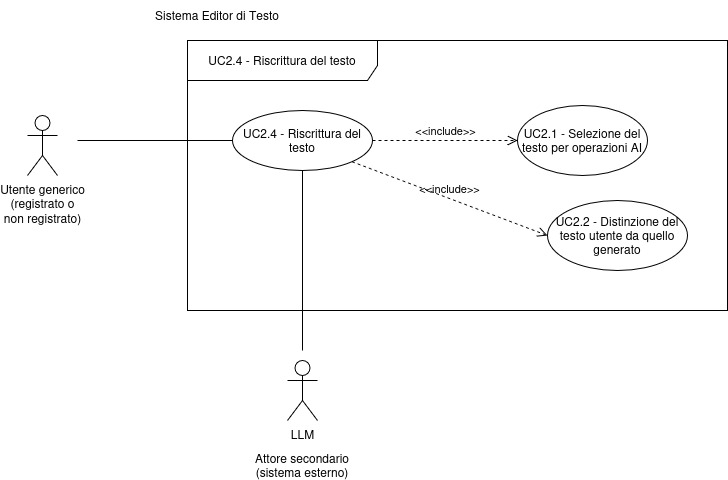
\includegraphics[width=0.8\textwidth]{../UCimg/UC2.4_riscrittura.jpg}
    \caption{Diagramma del caso d'uso UC-2.4}
    \label{fig:uc2.4}
\end{figure}

\subsubsection{UC-2.5 - Traduzione del testo in inglese (caso generico principale)}
\begin{itemize}
    \item \textbf{Attore principale}: Utente generico
    \item \textbf{Descrizione}: Traduzione automatica del testo nella lingua inglese (lingua predefinita)
    \item \textbf{Precondizioni}: È presente testo nell'editor (completo o selezionato)
    \item \textbf{Postcondizioni}: Il testo viene tradotto in lingua inglese
    \item \textbf{Scenario principale}:
        \begin{itemize}
            \item L'utente seleziona il testo da tradurre (opzionale)
            \item L'utente clicca sul comando "Traduci"
            \item Il sistema seleziona automaticamente l'inglese come lingua di destinazione (predefinita)
            \item Il sistema invia il testo al LLM
            \item Il sistema mostra la traduzione generata
            \item L'utente può scegliere di sostituire il testo originale o mantenere entrambe le versioni
        \end{itemize}
    \item \textbf{Estensioni}:
        \begin{itemize}
            \item Il testo è già in lingua inglese:
                \begin{enumerate}
                    \item Il sistema avvisa l'utente
                    \item L'operazione può essere annullata
                \end{enumerate}
        \end{itemize}
\end{itemize}

\subsubsection{UC-2.5.1 - Traduzione del testo in Spagnolo}
\begin{itemize}
    \item \textbf{Attore principale}: Utente generico
    \item \textbf{Descrizione}: Traduzione automatica del testo nella lingua spagnola %FORSE SI POTREBBE OMETTERE LA DESCRIZIONE PER I SOTTOCASI (molte ripetizioni)
    \item \textbf{Precondizioni}: È presente testo nell'editor (completo o selezionato)
    \item \textbf{Postcondizioni}: Il testo viene tradotto in lingua spagnola
    \item \textbf{Scenario principale}:
        \begin{itemize}
            \item L'utente seleziona il testo da tradurre
            \item L'utente clicca sul comando "Traduci"
            \item L'utente seleziona "Spagnolo" come lingua di destinazione
            \item Il sistema invia il testo al LLM per traduzione in spagnolo
            \item Il sistema mostra la traduzione generata
            \item L'utente può scegliere di sostituire il testo originale o mantenere entrambe le versioni
        \end{itemize}
    \item \textbf{Estensioni}:
        \begin{itemize}
            \item Il testo è già in spagnolo:
                \begin{enumerate}
                    \item Il sistema avvisa l'utente
                    \item L'operazione può essere annullata
                \end{enumerate}
        \end{itemize}
\end{itemize}

\subsubsection{UC-2.5.2 - Traduzione del testo in Francese}
\begin{itemize}
    \item \textbf{Attore principale}: Utente generico
    \item \textbf{Descrizione}: Traduzione automatica del testo nella lingua francese
    \item \textbf{Precondizioni}: È presente testo nell'editor (completo o selezionato)
    \item \textbf{Postcondizioni}: Il testo viene tradotto in lingua francese
    \item \textbf{Scenario principale}:
        \begin{itemize}
            \item L'utente seleziona il testo da tradurre (opzionale)
            \item L'utente clicca sul comando "Traduci"
            \item L'utente seleziona "Francese" come lingua di destinazione
            \item Il sistema invia il testo al LLM per traduzione in francese
            \item Il sistema mostra la traduzione generata
            \item L'utente può scegliere di sostituire il testo originale o mantenere entrambe le versioni
        \end{itemize}
    \item \textbf{Estensioni}:
        \begin{itemize}
            \item Il testo è già in francese:
                \begin{enumerate}
                    \item Il sistema avvisa l'utente
                    \item L'operazione può essere annullata
                \end{enumerate}
        \end{itemize}
\end{itemize}

\subsubsection{UC-2.5.3 - Traduzione del testo in Tedesco}
\begin{itemize}
    \item \textbf{Attore principale}: Utente generico
    \item \textbf{Descrizione}: Traduzione automatica del testo nella lingua tedesca
    \item \textbf{Precondizioni}: È presente testo nell'editor (completo o selezionato)
    \item \textbf{Postcondizioni}: Il testo viene tradotto in lingua tedesca
    \item \textbf{Scenario principale}:
        \begin{itemize}
            \item L'utente seleziona il testo da tradurre
            \item L'utente clicca sul comando "Traduci"
            \item L'utente seleziona "Tedesco" como lingua di destinazione
            \item Il sistema invia il testo al LLM per traduzione in tedesco
            \item Il sistema mostra la traduzione generata
            \item L'utente può scegliere di sostituire il testo originale o mantenere entrambe le versioni
        \end{itemize}
    \item \textbf{Estensioni}:
        \begin{itemize}
            \item Il testo è già in tedesco:
                \begin{enumerate}
                    \item Il sistema avvisa l'utente
                    \item L'operazione può essere annullata
                \end{enumerate}
        \end{itemize}
\end{itemize}

\subsubsection{UC-2.5.4 - Traduzione del testo in Cinese Mandarino}
\begin{itemize}
    \item \textbf{Attore principale}: Utente generico
    \item \textbf{Descrizione}: Traduzione automatica del testo nella lingua cinese mandarino
    \item \textbf{Precondizioni}: È presente testo nell'editor (completo o selezionato)
    \item \textbf{Postcondizioni}: Il testo viene tradotto in lingua cinese mandarino
    \item \textbf{Scenario principale}:
        \begin{itemize}
            \item L'utente seleziona il testo da tradurre
            \item L'utente clicca sul comando "Traduci"
            \item L'utente seleziona "Cinese Mandarino" come lingua di destinazione
            \item Il sistema invia il testo al LLM per traduzione in cinese mandarino
            \item Il sistema mostra la traduzione generata
            \item L'utente può scegliere di sostituire il testo originale o mantenere entrambe le versioni
        \end{itemize}
    \item \textbf{Estensioni}:
        \begin{itemize}
            \item Il testo è già in cinese mandarino:
                \begin{enumerate}
                    \item Il sistema avvisa l'utente
                    \item L'operazione può essere annullata
                \end{enumerate}
        \end{itemize}
\end{itemize}

\subsubsection{UC-2.5.5 - Traduzione del testo in Italiano}
\begin{itemize}
    \item \textbf{Attore principale}: Utente generico
    \item \textbf{Descrizione}: Traduzione automatica del testo nella lingua Italiana
    \item \textbf{Precondizioni}: È presente testo nell'editor (completo o selezionato)
    \item \textbf{Postcondizioni}: Il testo viene tradotto in lingua Italiana
    \item \textbf{Scenario principale}:
        \begin{itemize}
            \item L'utente seleziona il testo da tradurre
            \item L'utente clicca sul comando "Traduci"
            \item L'utente seleziona "Italiano" come lingua di destinazione
            \item Il sistema invia il testo al LLM per traduzione in Italiano
            \item Il sistema mostra la traduzione generata
            \item L'utente può scegliere di sostituire il testo originale o mantenere entrambe le versioni
        \end{itemize}
    \item \textbf{Estensioni}:
        \begin{itemize}
            \item Il testo è già in Italiano:
                \begin{enumerate}
                    \item Il sistema avvisa l'utente
                    \item L'operazione può essere annullata
                \end{enumerate}
        \end{itemize}
\end{itemize}


\subsubsection{UC-2.5.6 - Gestione del Testo Tradotto Generato}
\begin{itemize}
    \item \textbf{Attore principale}: Utente generico
    \item \textbf{Descrizione}: Sistema di visualizzazione e gestione del testo tradotto all'interno dell'editor
    \item \textbf{Precondizioni}: È stata generata una traduzione e il sistema mostra sia il testo originale che la traduzione
    \item \textbf{Postcondizioni}: Il testo tradotto viene inserito nell'editor con un formato distintivo
    \item \textbf{Scenario principale}:
        \begin{itemize}
            \item L'utente ha richiesto una traduzione e la traduzione è stata generata correttamente
            \item Il sistema mostra la traduzione nell'editor di testo sotto il testo originale, distinguendo le due porzioni di testo con:
                \begin{enumerate}
                    \item Una riga separatrice orizzontale (---) o altro elemento separatore
                    \item Commento iniziale in corsivo e grigio: Generato da AI - Traduzione - [data]
                    \item Sfondo colorato leggero (es. azzurro chiaro per traduzioni, verde chiaro per riassunti)
                    \item un’area apposita (box) identificativa
                    \item colore del testo generato diverso dal colore del testo dell’utente
                \end{enumerate}
            \item Il testo originale rimane invariato nella sua posizione
            \item L'utente può modificare, spostare o eliminare entrambe le versioni
        \end{itemize}
\end{itemize}

% DIAGRAMMA
\begin{figure}[H]
    \centering
    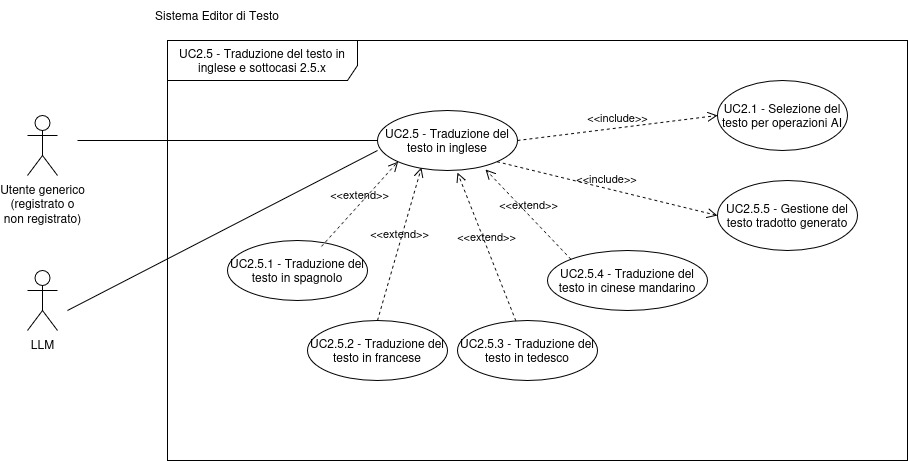
\includegraphics[width=0.8\textwidth]{../UCimg/UC2.5_traduzione.jpg}
    \caption{Diagramma dei casi d'uso UC-2.5.*}
    \label{fig:uc2.5}
\end{figure}

\subsubsection{UC-2.6 - Correzione grammaticale}
\begin{itemize}
    \item \textbf{Attore principale}: Utente generico
    \item \textbf{Descrizione}: Rilevamento e correzione automatica di errori grammaticali, ortografici e di punteggiatura
    \item \textbf{Precondizioni}: È presente testo nell'editor (completo o selezionato)
    \item \textbf{Postcondizioni}: Gli errori grammaticali vengono corretti
    \item \textbf{Scenario principale}:
        \begin{itemize}
            \item L'utente seleziona il testo da correggere
            \item L'utente clicca sul comando "Correggi"
            \item Il sistema invia il testo al LLM
            \item Il sistema mostra il testo corretto evidenziando le modifiche (opzionale)
            \item L'utente conferma le correzioni
        \end{itemize}
    \item \textbf{Estensioni}:
        \begin{itemize}
            \item L'LLM non è disponibile o dà errore:
                \begin{enumerate}
                    \item Il sistema mostra un messaggio di errore
                    \item Suggerisce di riprovare più tardi
                \end{enumerate}
        \end{itemize}
\end{itemize}

% DIAGRAMMA
\begin{figure}[H]
    \centering
    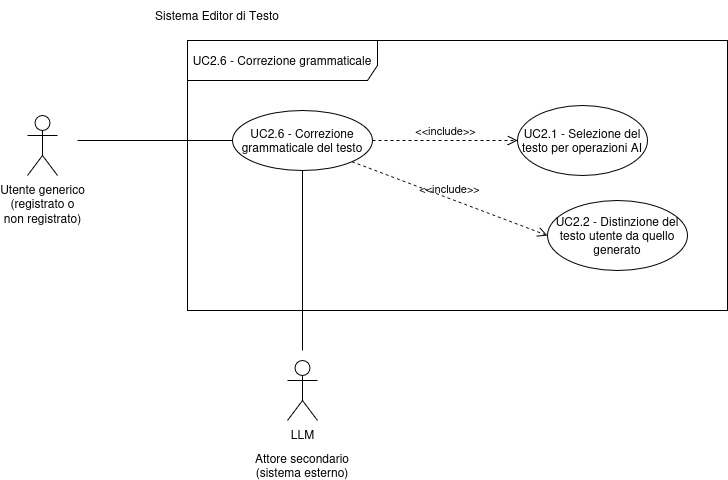
\includegraphics[width=0.8\textwidth]{../UCimg/UC2.6_correzione.jpg}
    \caption{Diagramma del caso d'uso UC-2.6}
    \label{fig:uc2.6}
\end{figure}

\subsubsection{UC-2.7 - Critica testuale con i 6 Cappelli: Cappello Bianco}
\begin{itemize}
    \item \textbf{Attore principale}: Utente generico
    \item \textbf{Descrizione}: Analisi oggettiva e fattuale del testo basata sul modello del Cappello Bianco di De Bono
    \item \textbf{Precondizioni}: È presente testo selezionato nell'editor
    \item \textbf{Postcondizioni}: Viene generata un'analisi oggettiva e fattuale del testo
    \item \textbf{Scenario principale}:
        \begin{itemize}
            \item L'utente seleziona il testo da analizzare (opzionale)
            \item L'utente clicca sul menu "Analisi critica"
            \item Il sistema seleziona automaticamente il Cappello Bianco come modalità predefinita oppure l'utente sceglie "Cappello Bianco" dal menu analisi
            \item Il sistema invia il testo al LLM con focus su dati, fatti e informazioni oggettive
            \item Il sistema mostra l'analisi fattuale generata
        \end{itemize}
    \item \textbf{Estensioni}:
        \begin{itemize}
            \item Il testo è troppo breve per un'analisi significativa:
                \begin{enumerate}
                    \item Il sistema avvisa l'utente e suggerisce di aggiungere contenuto
                \end{enumerate}
        \end{itemize}
\end{itemize}

\subsubsection{UC-2.7.1 - Analisi Cappello Rosso}
\begin{itemize}
    \item \textbf{Attore principale}: Utente generico
    \item \textbf{Descrizione}: Analisi emotiva e intuitiva del testo basata sul modello del Cappello Rosso di De Bono
    \item \textbf{Precondizioni}: È presente testo selezionato nell'editor
    \item \textbf{Postcondizioni}: Viene generata un'analisi emotiva e intuitiva del testo
    \item \textbf{Scenario principale}:
        \begin{itemize}
            \item L'utente seleziona il testo da analizzare (opzionale)
            \item L'utente sceglie "Cappello Rosso" dal menu analisi
            \item Il sistema invia il testo al LLM con focus su emozioni, sentimenti e reazioni intuitive
            \item Il sistema mostra l'analisi emotiva generata
        \end{itemize}
\end{itemize}

\subsubsection{UC-2.7.2 - Analisi Cappello Nero}
\begin{itemize}
    \item \textbf{Attore principale}: Utente generico
    \item \textbf{Descrizione}: Analisi critica e cautelativa del testo basata sul modello del Cappello Nero di De Bono
    \item \textbf{Precondizioni}: È presente testo selezionato nell'editor
    \item \textbf{Postcondizioni}: Viene generata un'analisi critica e cautelativa del testo
    \item \textbf{Scenario principale}:
        \begin{itemize}
            \item L'utente seleziona il testo da analizzare (opzionale)
            \item L'utente sceglie "Cappello Nero" dal menu analisi
            \item Il sistema invia il testo al LLM con focus su criticità, rischi e punti deboli
            \item Il sistema mostra l'analisi critica generata
        \end{itemize}
\end{itemize}

\subsubsection{UC-2.7.3 - Analisi Cappello Giallo}
\begin{itemize}
    \item \textbf{Attore principale}: Utente generico
    \item \textbf{Descrizione}: Analisi ottimistica e costruttiva del testo basata sul modello del Cappello Giallo di De Bono
    \item \textbf{Precondizioni}: È presente testo selezionato nell'editor
    \item \textbf{Postcondizioni}: Viene generata un'analisi ottimistica e costruttiva del testo
    \item \textbf{Scenario principale}:
        \begin{itemize}
            \item L'utente seleziona il testo da analizzare (opzionale)
            \item L'utente sceglie "Cappello Giallo" dal menu analisi
            \item Il sistema invia il testo al LLM con focus su benefici, opportunità e aspetti positivi
            \item Il sistema mostra l'analisi ottimistica generata
        \end{itemize}
\end{itemize}

\subsubsection{UC-2.7.4 - Analisi Cappello Verde}
\begin{itemize}
    \item \textbf{Attore principale}: Utente generico
    \item \textbf{Descrizione}: Analisi creativa e innovativa del testo basata sul modello del Cappello Verde di De Bono
    \item \textbf{Precondizioni}: È presente testo selezionato nell'editor
    \item \textbf{Postcondizioni}: Viene generata un'analisi creativa e innovativa del testo
    \item \textbf{Scenario principale}:
        \begin{itemize}
            \item L'utente seleziona il testo da analizzare (opzionale)
            \item L'utente sceglie "Cappello Verde" dal menu analisi
            \item Il sistema invia il testo al LLM con focus su idee creative, alternative e innovazioni
            \item Il sistema mostra l'analisi creativa generata
        \end{itemize}
\end{itemize}

\subsubsection{UC-2.7.5 - Analisi Cappello Blu}
\begin{itemize}
    \item \textbf{Attore principale}: Utente generico
    \item \textbf{Descrizione}: Analisi processuale e organizzativa del testo basata sul modello del Cappello Blu di De Bono
    \item \textbf{Precondizioni}: È presente testo selezionato nell'editor
    \item \textbf{Postcondizioni}: Viene generata un'analisi processuale e organizzativa del testo
    \item \textbf{Scenario principale}:
        \begin{itemize}
            \item L'utente seleziona il testo da analizzare (opzionale)
            \item L'utente sceglie "Cappello Blu" dal menu analisi
            \item Il sistema invia il testo al LLM con focus su struttura, processo e organizzazione
            \item Il sistema mostra l'analisi processuale generata
        \end{itemize}
\end{itemize}

\subsubsection{UC-2.7.6 - Gestione dell'Analisi Critica Generata}
\begin{itemize}
    \item \textbf{Attore principale}: Utente generico
    \item \textbf{Descrizione}: Sistema di visualizzazione e organizzazione delle analisi critiche generate nel documento
    \item \textbf{Precondizioni}: È stata generata un'analisi critica
    \item \textbf{Postcondizioni}: L'analisi critica viene inserita nell'editor con formattazione distintiva
    \item \textbf{Scenario principale}:
        \begin{itemize}
            \item Il sistema mostra l'analisi critica generata nell'editor di testo
            \item Il sistema inserisce l'analisi sotto il testo analizzato distinguendola dal testo tramite:
                \begin{enumerate}
                    \item Una riga separatrice orizzontale (---) o altro elemento separatore
                    \item Commento iniziale in corsivo e grigio: Generato da AI - Analisi [cappello] - [data]
                    \item Sfondo colorato leggero (es. azzurro chiaro per traduzioni, verde chiaro per riassunti) (opzionale)
                    \item un’area apposita (box) identificativa
                    \item colore del testo generato diverso dal colore del testo dell’utente (opzionale)
                \end{enumerate}
            \item Il testo originale analizzato rimane invariato nella sua posizione
            \item L'utente può modificare, spostare o eliminare l'analisi generata
        \end{itemize}
\end{itemize}

% DIAGRAMMA
\begin{figure}[H]
    \centering
    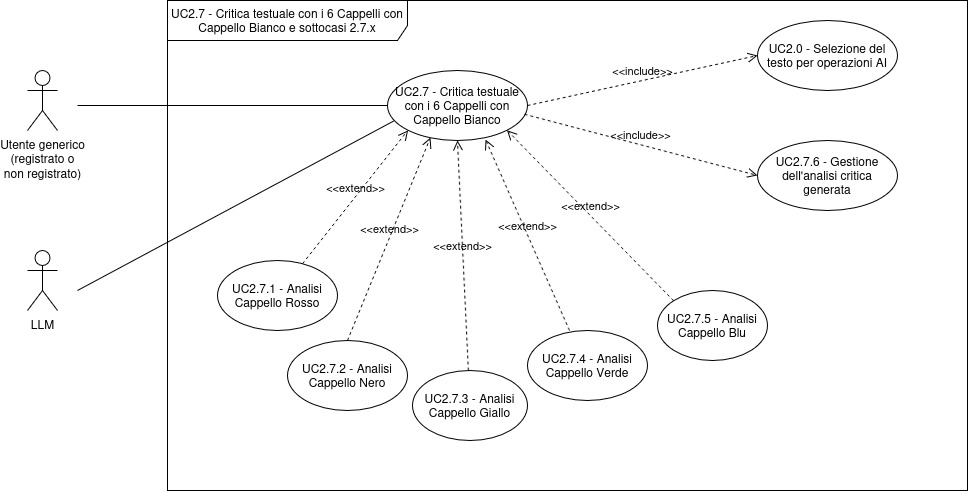
\includegraphics[width=0.8\textwidth]{../UCimg/UC2.7_6cappelli.jpg}
    \caption{Diagramma dei casi d'uso UC-2.7.*}
    \label{fig:uc2.7}
\end{figure}

\subsubsection{UC-2.8 - Generazione di testo (Distant Writing)}
\begin{itemize}
    \item \textbf{Attore principale}: Utente generico
    \item \textbf{Descrizione}: Creazione di nuovo testo a partire da un prompt descrittivo fornito dall'utente
    \item \textbf{Precondizioni}: L'editor è aperto e pronto per la scrittura
    \item \textbf{Postcondizioni}: Viene generato un nuovo testo basato sul prompt dell'utente e inserito nell'editor con formattazione che ne identifica l'origine AI
    \item \textbf{Scenario principale}:
        \begin{itemize}
            \item L'utente si posiziona nel punto del documento dove vuole inserire il testo generato
            \item L'utente inserisce un prompt descrivendo il testo desiderato tramite:
                \begin{enumerate}
                    \item Chatbox dedicata nell'interfaccia
                    \item Comando rapido \textit{/genera} seguito dal prompt
                \end{enumerate}
            \item Il sistema invia il prompt al LLM
            \item Il sistema inserisce il testo generato nell'editor di testo nel punto dove l'utente si è posizionato
            \item Il testo generato è distinto da altro testo presente nell'editor tramite:
                \begin{enumerate}
                    \item Una riga separatrice orizzontale (---) o altro elemento separatore
                    \item Intestazione descrittiva in corsivo: Generato da AI - Testo generato da: "[estratto prompt]" - [data/ora]
                    \item Sfondo colorato leggero (es. azzurro chiaro per traduzioni, verde chiaro per riassunti) (opzionale)
                    \item un’area apposita (box) identificativa
                    \item colore del testo generato diverso dal colore del testo dell’utente (opzionale)
                \end{enumerate}
            \item L'utente può modificare il testo generato
        \end{itemize}
    \item \textbf{Estensioni}:
        \begin{itemize}
            \item L'utente fornisce un prompt troppo vago o incompleto (opzionale):
                \begin{enumerate}
                    \item Il sistema offre esempi di prompt efficaci basati sul contesto corrente (opzionale)
                \end{enumerate}
            \item Il testo generato non soddisfa l'utente:
                \begin{enumerate}
                    \item L'utente può richiedere una rigenerazione con modifiche al prompt
                    \item Ogni rigenerazione viene trattata come una nuova generazione separata nell'editor
                    \item Le generazioni precedenti vengono comunque mantenute (salvo eliminazione o modifica da parte dell'utente)
                \end{enumerate}
        \end{itemize}
\end{itemize}

% DIAGRAMMA
\begin{figure}[H]
    \centering
    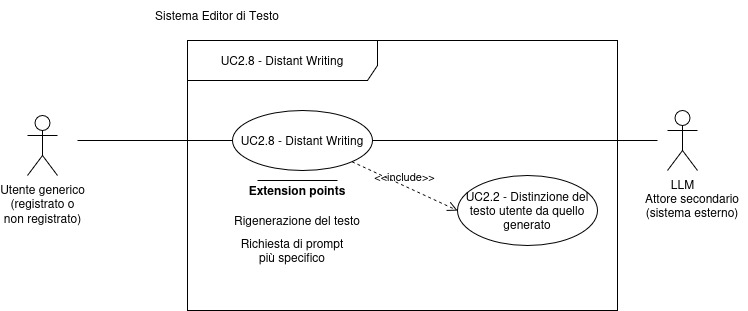
\includegraphics[width=0.8\textwidth]{../UCimg/UC2.8_distantWriting.jpg}
    \caption{Diagramma del caso d'uso UC-2.8}
    \label{fig:uc2.8}
\end{figure}

\subsubsection{UC-2.9 - Generazione grafici e tabelle (opzionale)}
\begin{itemize}
    \item \textbf{Attore principale}: Utente generico
    \item \textbf{Descrizione}: Creazione automatica di grafici e tabelle basate su dati descritti nel testo
    \item \textbf{Precondizioni}: È presente testo descrittivo nell'editor
    \item \textbf{Postcondizioni}: Viene generato un grafico o tabella basato sul testo
    \item \textbf{Scenario principale}:
        \begin{itemize}
            \item L'utente seleziona il testo descrittivo dei dati
            \item L'utente clicca sul bottone "Genera grafico"
            \item L'utente specifica il tipo di grafico/tabella desiderato
            \item Il sistema invia la richiesta al LLM
            \item Il sistema mostra il grafico/tabella generato
        \end{itemize}
    \item \textbf{Estensioni}:
        \begin{itemize}
            \item Il testo non contiene dati strutturati sufficienti:
                \begin{enumerate}
                    \item Il sistema segnala l'impossibilità di generare il grafico
                \end{enumerate}
            \item Il grafico generato non è leggibile:
                \begin{enumerate}
                    \item L'utente può richiedere una rigenerazione con parametri diversi
                \end{enumerate}
        \end{itemize}
\end{itemize}


\subsubsection{UC-2.10 - Generazione mappe concettuali (opzionale)}
\begin{itemize}
    \item \textbf{Attore principale}: Utente generico
    \item \textbf{Descrizione}: Creazione di mappe concettuali per visualizzare e organizzare le relazioni tra concetti nel testo
    \item \textbf{Precondizioni}: È presente testo nell'editor (completo o selezionato)
    \item \textbf{Postcondizioni}: Viene generata una mappa concettuale del testo
    \item \textbf{Scenario principale}:
        \begin{itemize}
            \item L'utente seleziona il testo da visualizzare come mappa
            \item L'utente clicca su "Genera mappa concettuale"
            \item Il sistema invia il testo al LLM
            \item Il sistema mostra la mappa concettuale generata
        \end{itemize}
    \item \textbf{Estensioni}:
        \begin{itemize}
            \item Il testo è troppo complesso per una singola mappa:
                \begin{enumerate}
                    \item Il sistema genera mappe multiple o una mappa semplificata o segnala l'impossibilità di generarla
                \end{enumerate}
            \item La mappa generata non è chiara:
                \begin{enumerate}
                    \item L'utente può richiedere una riorganizzazione con focus diversi
                \end{enumerate}
            \item Problemi di visualizzazione della mappa:
                \begin{enumerate}
                    \item Il sistema offre alternative testuali o esportazione in altri formati o dà errore
                \end{enumerate}
        \end{itemize}
\end{itemize}

\subsubsection{UC-2.11 - Generazione formule matematiche (opzionale)}
\begin{itemize}
    \item \textbf{Attore principale}: Utente generico
    \item \textbf{Descrizione}: Creazione automatica di formule matematiche basate su descrizioni testuali di problemi
    \item \textbf{Precondizioni}: È presente testo descrittivo di problemi matematici
    \item \textbf{Postcondizioni}: Vengono generate formule matematiche appropriate
    \item \textbf{Scenario principale}:
        \begin{itemize}
            \item L'utente seleziona il testo descrittivo del problema
            \item L'utente clicca su "Genera formule"
            \item Il sistema invia la richiesta al LLM
            \item Il sistema mostra le formule matematiche generate in formato LaTeX o simili
        \end{itemize}
    \item \textbf{Estensioni}:
        \begin{itemize}
            \item Le formule generate contengono errori:
                \begin{enumerate}
                    \item L'utente può correggere manualmente o richiedere una rigenerazione
                \end{enumerate}
            \item Il sistema non supporta simboli matematici complessi:
                \begin{enumerate}
                    \item Il sistema segnala le limitazioni e suggerisce alternative
                \end{enumerate}
        \end{itemize}
\end{itemize}

% DIAGRAMMA PER CASI D'USO OPZIONALI
\begin{figure}[H]
    \centering
    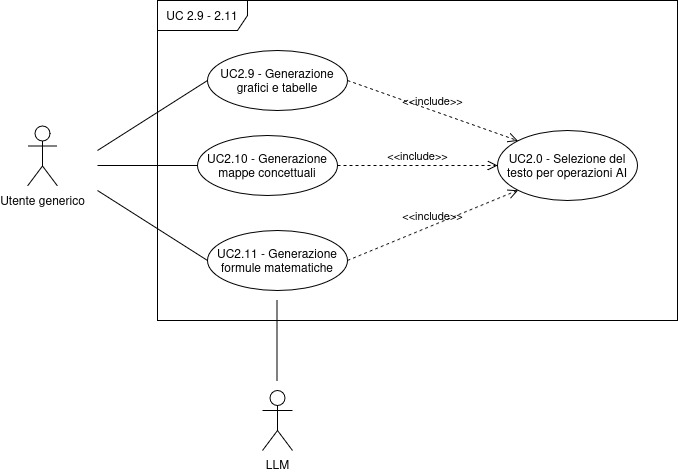
\includegraphics[width=0.8\textwidth]{../UCimg/UC2.9_11_opzionali.jpg}
    \caption{Diagramma dei casi d'uso UC-2.9, UC-2.10, UC2.11 (opzionali)}
    \label{fig:uc2.9}
\end{figure}

\newpage

\subsection{Macroarea 3 - Persistenza: Caricamento}
\subsubsection{UC-3.0 - Caricamento file}
\begin{itemize}
    \item \textbf{Attore principale}: Utente generico
    \item \textbf{Descrizione}: Permettere all'utente di caricare un documento nell'editor
    \item \textbf{Precondizioni}: L'utente ha un file che vuole caricare nell'editor
    \item \textbf{Postcondizioni}: L'utente ha caricato con successo il file nell'editor
    \item \textbf{Scenario principale}:
        \begin{itemize}
            \item Utente vuole caricare un file
            \item Utente clicca il pulsante per caricare il file
            \item Utente sceglie tra due opzioni: trascina file e esplora file
            \item Utente carica il documento
        \end{itemize}
\end{itemize}

\subsubsection{UC-3.0.0 - Opzione trascina file}
\begin{itemize}
    \item \textbf{Attore principale}: Utente generico
    \item \textbf{Descrizione}: Utente trascina il file nella finestra per caricare file
    \item \textbf{Precondizioni}: Utente clicca tasto per trascinare file
    \item \textbf{Postcondizioni}: Utente ha trascinato file
    \item \textbf{Scenario principale}:
        \begin{itemize}
            \item Utente sceglie opzione trascina file
            \item Utente trascina file
            \item Utente ha caricato il file
        \end{itemize}
\end{itemize}

\subsubsection{UC-3.0.1 - Opzione esplora file}
\begin{itemize}
    \item \textbf{Attore principale}: Utente generico
    \item \textbf{Descrizione}: Utente vede i propri file e ne sceglie uno da caricare
    \item \textbf{Precondizioni}: Utente clicca tasto per aprire esplora file
    \item \textbf{Postcondizioni}: Utente ha scelto un file
    \item \textbf{Scenario principale}:
        \begin{itemize}
            \item Utente sceglie opzione esplora file
            \item Utente trascina file
            \item Utente ha caricato il file
        \end{itemize}
\end{itemize}

\begin{figure}[H]
    \centering
    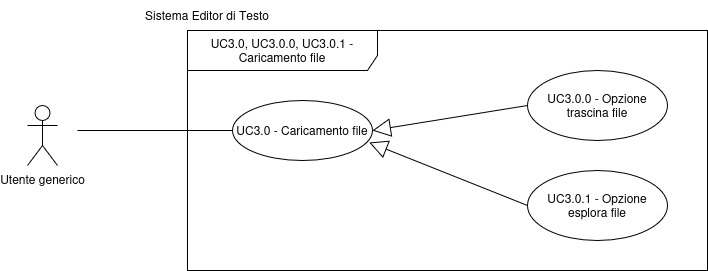
\includegraphics[width=0.8\textwidth]{../UCimg/UC3.0_caricamento.jpg}
    \caption{Diagramma dei casi d'uso UC-3.0, 3.0.0, 3.0.1}
    \label{fig:uc3.0}
\end{figure}

\subsubsection{UC-3.1 - Errore: Formato file non supportato}
\begin{itemize}
    \item \textbf{Attore principale}: Utente generico
    \item \textbf{Descrizione}: L'utente prova a caricare un documento ma è di un formato non supportato
    \item \textbf{Precondizioni}: Il file caricato è di un formato non supportato
    \item \textbf{Postcondizioni}: Appare il messaggio di errore "Formato non supportato"
\end{itemize}

\subsubsection{UC-3.2 - Errore: File troppo grande}
\begin{itemize}
    \item \textbf{Attore principale}: Utente generico
    \item \textbf{Descrizione}: L'utente prova a caricare un documento ma è di dimensioni troppo grandi
    \item \textbf{Precondizioni}: Il file caricato è di dimensioni troppo grandi
    \item \textbf{Postcondizioni}: Appare il messaggio di errore "File troppo grande"
\end{itemize}

\subsubsection{UC-3.3 - Rimozione file caricato}
\begin{itemize}
    \item \textbf{Attore principale}: Utente generico
    \item \textbf{Descrizione}: utente vuole rimuovere un file che ha caricato
    \item \textbf{Precondizioni}: utente clicca tasto per rimuovere file caricato
    \item \textbf{Postcondizioni}: utente ha rimosso con successo il file
    \item \textbf{Scenario principale}:
        \begin{itemize}
            \item Utente clicca il pulsante rimuovi file
            \item Utente vede la schermata “Sei sicuro di voler rimuovere?”
            \item Utente preme si e rimuove con successo il file
        \end{itemize}
        \item \textbf{Estensioni}:
        \begin{itemize}
            \item Utente clicca no nella schermata “Sei sicuro di voler rimuovere?” e quindi il file non viene rimosso
        \end{itemize}
\end{itemize}

\begin{figure}[H]
    \centering
    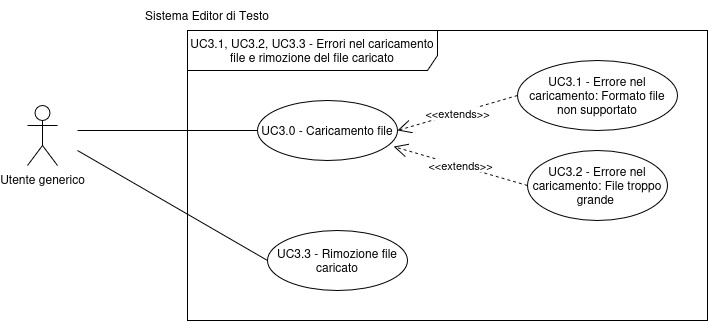
\includegraphics[width=0.8\textwidth]{../UCimg/UC3.1_3.2_3.3_errori.jpg}
    \caption{Diagramma dei casi d'uso UC-3.1, 3.2, 3.3}
    \label{fig:uc3.1}
\end{figure}

\newpage

\subsection{Macroarea 4 - Persistenza: Salvataggio}
\subsubsection{UC-4.0 - Esportazione dei file}
\begin{itemize}
    \item \textbf{Attore principale}: Utente generico
    \item \textbf{Descrizione}: Permettere all'utente di salvare il documento su cui ha lavorato
    \item \textbf{Precondizioni}: Testo scritto nell'editor di testo
    \item \textbf{Postcondizioni}: L'utente ha il documento salvato in locale
    \item \textbf{Scenario principale}:
        \begin{itemize}
            \item Utente scrive del testo
            \item Utente decide di esportare il documento
            \item Utente preme sul tasto esporta
            \item Utente ottiene una serie di opzioni per l'esportazione
        \end{itemize}
\end{itemize}
\begin{figure}[H]
    \centering
    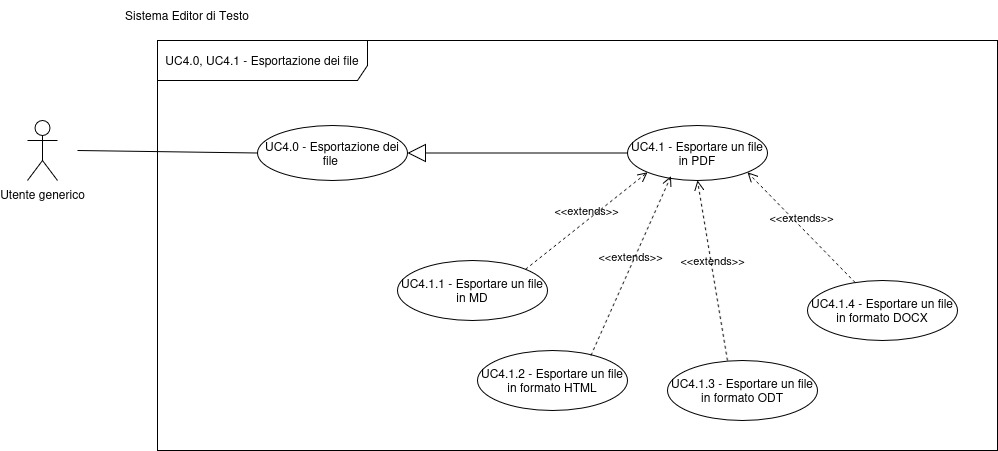
\includegraphics[width=0.8\textwidth]{../UCimg/UC4.0_esportazioneFile.jpg}
    \caption{Diagramma dei casi d'uso UC-4.0, UC-4.1, UC-4.1.*}
    \label{fig:uc4.0}
\end{figure}

\subsubsection{UC-4.1 - Esportare un file in PDF}
\begin{itemize}
    \item \textbf{Attore principale}: Utente generico
    \item \textbf{Descrizione}: Testo compilato salvato in locale sulla propria macchina in formato PDF
    \item \textbf{Precondizioni}: L'utente ha un documento che desidera scaricare
    \item \textbf{Postcondizioni}: L'utente ottiene un documento in formato PDF salvato localmente
    \item \textbf{Scenario principale}:
        \begin{itemize}
            \item Utente seleziona l'opzione "PDF" tra le opzioni di esportazione
            \item Il documento viene convertito in formato PDF
            \item Utente ottiene il documento salvato in PDF
        \end{itemize}
\end{itemize}

\subsubsection{UC-4.1.1 - Esportare un file in MD}
\begin{itemize}
    \item \textbf{Attore principale}: Utente generico
    \item \textbf{Descrizione}: Testo compilato salvato in locale sulla propria macchina in formato testuale
    \item \textbf{Precondizioni}: L'utente ha un documento che desidera scaricare
    \item \textbf{Postcondizioni}: L'utente ottiene un documento in formato MD salvato localmente
    \item \textbf{Scenario principale}:
        \begin{itemize}
            \item Utente seleziona opzione "src" tra le opzioni di esportazione
            \item Il documento viene salvato in formato MD
        \end{itemize}
\end{itemize}

\subsubsection{UC-4.1.2 - Esportare un file in formato HTML}
\begin{itemize}
    \item \textbf{Attore principale}: Utente generico
    \item \textbf{Descrizione}: Genera del codice HTML dal testo Markdown
    \item \textbf{Precondizioni}: L'utente ha un documento non vuoto
    \item \textbf{Postcondizioni}: L'utente ottiene un file .HTML in cui viene convertito il testo Markdown in codice HTML
    \item \textbf{Scenario principale}:
        \begin{itemize}
            \item Utente seleziona opzione "HTML" tra le opzioni di esportazione
            \item Il documento viene convertito in formato HTML
            \item Utente riceve il documento in formato HTML
        \end{itemize}
\end{itemize}

\subsubsection{UC-4.1.3 - Esportare un file in formato ODT}
\begin{itemize}
    \item \textbf{Attore principale}: Utente generico
    \item \textbf{Descrizione}: Genera documenti compatibili con popolari editor testuali
    \item \textbf{Precondizioni}: L'utente ha un documento non vuoto
    \item \textbf{Postcondizioni}: L'utente ottiene un file .ODT salvato localmente
    \item \textbf{Scenario principale}:
        \begin{itemize}
            \item Utente seleziona opzione "ODT" tra le opzioni di esportazione
            \item Il documento viene convertito in formato ODT
            \item Utente riceve il documento in formato ODT
        \end{itemize}
\end{itemize}

\subsubsection{UC-4.1.4 - Esportare un file in formato DOCX}
\begin{itemize}
    \item \textbf{Attore principale}: Utente generico
    \item \textbf{Descrizione}: Genera documenti compatibili con Microsoft Word
    \item \textbf{Precondizioni}: L'utente ha un documento non vuoto
    \item \textbf{Postcondizioni}: L'utente ottiene un file .DOCX salvato localmente
    \item \textbf{Scenario principale}:
        \begin{itemize}
            \item Utente seleziona opzione "DOCX" tra le opzioni di esportazione
            \item Il documento viene convertito in formato DOCX
            \item Utente riceve il documento in formato DOCX
        \end{itemize}
\end{itemize}

\subsubsection{UC-4.2 - Esportare selezionate pagine del documento}
\begin{itemize}
    \item \textbf{Attore principale}: Utente generico
    \item \textbf{Descrizione}: Scaricare nel formato desiderato solo alcune pagine del documento
    \item \textbf{Precondizioni}: L'utente ha un documento non vuoto, con diverse pagine
    \item \textbf{Postcondizioni}: L'utente ottiene un file in formato a scelta con solo le pagine selezionate
    \item \textbf{Scenario principale}:
        \begin{itemize}
            \item Utente vuole scaricare solo selezionate pagine del documento da salvare
            \item Tra le opzioni di esportazione, elenca numericamente le pagine desiderate
            \item Seleziona modalità di esportazione
            \item Ottiene le pagine selezionate in un nuovo documento, salvato nel formato selezionato
        \end{itemize}
\end{itemize}

\subsubsection{UC-4.2.1 - Esportare un range pagine del documento}
\begin{itemize}
    \item \textbf{Attore principale}: Utente generico
    \item \textbf{Descrizione}: Scaricare nel formato desiderato solo un range di pagine del documento
    \item \textbf{Precondizioni}: L'utente ha un documento non vuoto, con diverse pagine
    \item \textbf{Postcondizioni}: L'utente ottiene un file in formato a scelta con solo il range di pagine selezionate
    \item \textbf{Scenario principale}:
        \begin{itemize}
            \item Utente vuole scaricare porzioni consecutive di un documento
            \item Utente seleziona la pagina di inizio e fine del range da scaricare
            \item Seleziona modalità di esportazione
            \item Ottiene le pagine selezionate in un nuovo documento, salvato nel formato selezionato
        \end{itemize}
\end{itemize}
\begin{figure}[H]
    \centering
    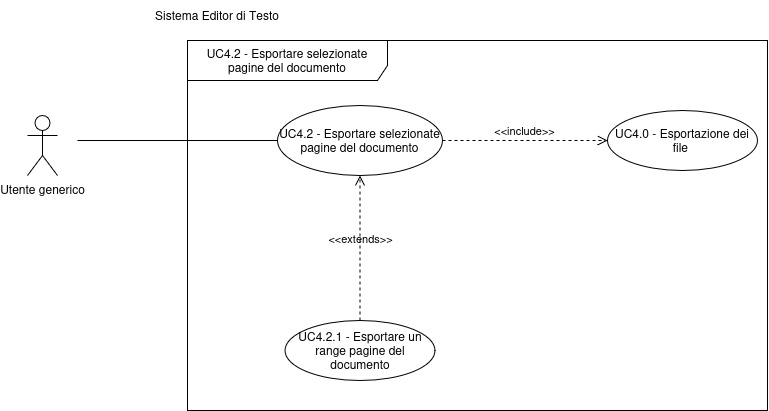
\includegraphics[width=0.8\textwidth]{../UCimg/UC4.2_esportazionePagine.jpg}
    \caption{Diagramma dei casi d'uso UC-4.2, UC-4.2.1}
    \label{fig:uc4.2}
\end{figure}

\subsubsection{UC-4.3 - Stampare il documento}
\begin{itemize}
    \item \textbf{Attore principale}: Utente generico
    \item \textbf{Descrizione}: Utente desidera stampare il documento senza doverlo prima esportare
    \item \textbf{Precondizioni}: L'utente ha un documento aperto
    \item \textbf{Postcondizioni}: L'utente ottiene il documento stampato
    \item \textbf{Scenario principale}:
        \begin{itemize}
            \item Utente ha un documento aperto che desidera stampare
            \item Utente preme un pulsante "stampa"
            \item Utente ha accesso alle opzioni di stampa offerte dal suo browser
            \item Utente ritorna al proprio documento una volta completata l'operazione
        \end{itemize}
\end{itemize}

\subsubsection{UC-4.3.1 - Stampare selezionate pagine del documento}
\begin{itemize}
    \item \textbf{Attore principale}: Utente generico
    \item \textbf{Descrizione}: Utente desidera stampare solo alcune pagine del documento
    \item \textbf{Precondizioni}: L'utente ha un documento aperto
    \item \textbf{Postcondizioni}: L'utente ottiene il documento stampato
    \item \textbf{Scenario principale}:
        \begin{itemize}
            \item Utente ha un documento aperto che desidera stampare
            \item Utente preme un pulsante "stampa"
            \item Utente ha accesso alle opzioni di stampa offerte dal suo browser
            \item Utente ha la possibilità di selezionare le pagine che desidera stampare
            \item Utente ritorna al proprio documento una volta completata l'operazione
        \end{itemize}
\end{itemize}
\begin{figure}[H]
    \centering
    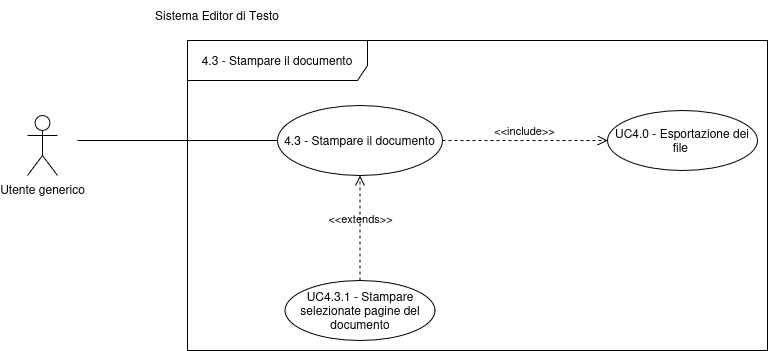
\includegraphics[width=0.8\textwidth]{../UCimg/UC4.3_stampa.jpg}
    \caption{Diagramma dei casi d'uso UC-4.3, UC-4.3.1}
    \label{fig:uc4.3}
\end{figure}

\newpage

\subsection{Macroarea 5 - Autenticazione (opzionale)}
\subsubsection{UC-5.0 - Login}
\begin{itemize}
    \item \textbf{Attore principale}: Utente non autenticato
    \item \textbf{Descrizione}: Permette all'utente di accedere al proprio account, rendendo così disponibili funzionalità di salvataggio, modifica e cancellazione di documenti nel db, salvati a nome dell'utente
    \item \textbf{Precondizioni}: L'utente è già registrato presso il sistema
    \item \textbf{Postcondizioni}: All'utente è permesso accedere al suo account nel sistema
    \item \textbf{Scenario principale}:
        \begin{itemize}
            \item L'utente accede al sistema
            \item L'utente seleziona la funzionalità Login
            \item L'utente inserisce un username ed una password univoci nel sistema
            \item All'utente viene permesso l'accesso
        \end{itemize}
    \item \textbf{Estensioni}:
        \begin{itemize}
            \item L'utente inserisce un username non presente nel db:
                \begin{enumerate}
                    \item All'utente non viene garantito l'accesso
                    \item Il sistema avvisa l'utente di aver inserito un username inesistente
                \end{enumerate}
            \item L'utente inserisce un username esistente ma la password sbagliata:
                \begin{enumerate}
                    \item All'utente non viene garantito l'accesso
                    \item Il sistema avvisa l'utente che la password inserita è errata
                \end{enumerate}
        \end{itemize}
\end{itemize}

\subsubsection{UC-5.1 - Registrazione}
\begin{itemize}
    \item \textbf{Attore principale}: Utente non autenticato
    \item \textbf{Descrizione}: L'utente potrà creare un nuovo account nel sistema accedendo così alle funzionalità di salvataggio, modifica e cancellazione di documenti nel db, salvati a nome dell'utente
    \item \textbf{Precondizioni}: L'utente non è ancora autenticato nel sistema
    \item \textbf{Postcondizioni}: L'utente possiede un account nel sistema individuato da un username ed una password
    \item \textbf{Scenario principale}:
        \begin{itemize}
            \item L'utente accede al sistema
            \item L'utente seleziona la funzionalità "Registrati"
            \item L'utente inserisce un username univoco nel sistema
            \item L'utente inserisce una password che rispetta i vincoli
        \end{itemize}
    \item \textbf{Estensioni}:
        \begin{itemize}
            \item L'utente inserisce un username già esistente nel sistema:
                \begin{enumerate}
                    \item L'utente non viene registrato
                    \item Il sistema avvisa l'utente che l'username inserito è già in utilizzo
                    \item Il sistema propone all'utente di effettuare il login o di scegliere un nuovo username
                \end{enumerate}
        \end{itemize}
\end{itemize}
\begin{figure}[H]
    \centering
    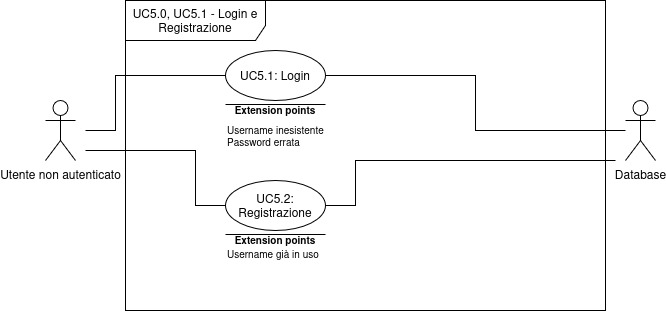
\includegraphics[width=0.8\textwidth]{../UCimg/UC5.0_5.1_login.jpg}
    \caption{Diagramma dei casi d'uso UC-5.0, UC-5.1}
    \label{fig:uc5.0}
\end{figure}

\subsubsection{UC-5.2 - Eliminazione dell'account}
\begin{itemize}
    \item \textbf{Attore principale}: Utente autenticato
    \item \textbf{Descrizione}: L'utente decide di eliminare il proprio account dal sistema
    \item \textbf{Precondizioni}: L'utente è autenticato nel sistema
    \item \textbf{Postcondizioni}: L'account dell'utente viene eliminato dal sistema e l'utente non potrà più accedere alle funzionalità relative alle sue note (vanno eliminate o impostate come anonime?)
    \item \textbf{Scenario principale}:
        \begin{itemize}
            \item L'utente accede al sistema
            \item L'utente seleziona l'opzione "Elimina account"
            \item Il sistema mostra un pop up di conferma della scelta
            \item L'utente accetta e viene sloggato
            \item Il sistema elimina dal db il nome utente e la password relative all'attore
        \end{itemize}
    \item \textbf{Estensioni}:
        \begin{itemize}
            \item L'utente seleziona "annulla" nel pop up di conferma:
                \begin{enumerate}
                    \item Il sistema non procede con l'eliminazione dell'account
                    \item Il pop up viene chiuso
                \end{enumerate}
        \end{itemize}
\end{itemize}

\subsubsection{UC-5.3 - Apertura file recenti}
\begin{itemize}
    \item \textbf{Attore principale}: Utente autenticato
    \item \textbf{Descrizione}: L'utente vuole aprire un file dal db creato in precedenza
    \item \textbf{Precondizioni}: L'utente è autenticato nel sistema
    \item \textbf{Postcondizioni}: L'utente continua a lavorare su una nota precedentemente salvata
    \item \textbf{Scenario principale}:
        \begin{itemize}
            \item L'utente accede al sistema
            \item L'utente seleziona l'opzione "Apri"
            \item Il sistema mostra un pop up in cui vengono mostrati i file salvati dall'utente attualmente loggato
            \item L'utente seleziona il file da aprire
            \item Il sistema recupera dal db la nota e la rende visibile
            \item L'utente può continuare a modificare la nota
        \end{itemize}
    \item \textbf{Estensioni}:
        \begin{itemize}
            \item L'utente seleziona "annulla" nel pop up di selezione:
                \begin{enumerate}
                    \item Il sistema non recupera nessuna nota dal db
                    \item Il pop up viene chiuso
                \end{enumerate}
        \end{itemize}
\end{itemize}

\subsubsection{UC-5.4 - Salvataggio file nel DataBase}
\begin{itemize}
    \item \textbf{Attore principale}: Utente autenticato
    \item \textbf{Descrizione}: L'utente vuole salvare la nota scritta nel database, senza scaricarla nel suo dispositivo corrente
    \item \textbf{Precondizioni}: L'utente ha scritto una nota ed ha eseguito l'accesso al sistema con il suo account
    \item \textbf{Postcondizioni}: Il sistema mantiene nel Database una copia della nota scritta, legandola all'account dell'utente
    \item \textbf{Scenario principale}:
        \begin{itemize}
            \item L'utente accede al sistema
            \item L'utente scrive del testo o ne genera con l'opzione relativa
            \item L'utente seleziona l'opzione di salvataggio
            \item Il sistema salva nel db una copia della nota dell'utente
        \end{itemize}
    \item \textbf{Estensioni}:
        \begin{itemize}
            \item L'utente non ha scritto o generato alcun testo:
                \begin{enumerate}
                    \item Il sistema avvisa che non può salvare note vuote
                    \item Il salvataggio non avviene
                \end{enumerate}
            \item L'utente non è autenticato:
                \begin{enumerate}
                    \item Il sistema avvisa che è necessario eseguire l'accesso per poter salvare nel db
                    \item Il sistema consiglia di eseguire l'accesso o esportare la nota in uno dei formati concessi
                \end{enumerate}
        \end{itemize}
\end{itemize}
\begin{figure}[H]
    \centering
    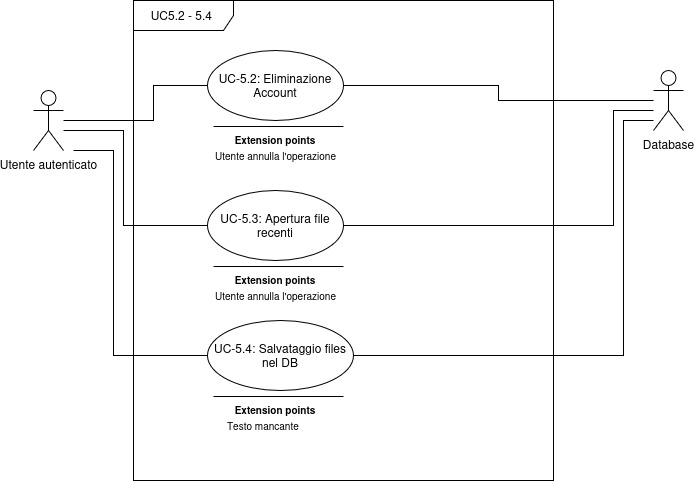
\includegraphics[width=0.8\textwidth]{../UCimg/UC5.2_5.4.jpg}
    \caption{Diagramma dei casi d'uso UC-5.2, UC-5.3, UC-5.4}
    \label{fig:uc5.2}
\end{figure}

\subsubsection{UC-5.5 - Logout}
\begin{itemize}
    \item \textbf{Attore principale}: Utente autenticato
    \item \textbf{Descrizione}: L'utente desidera terminare la propria sessione
    \item \textbf{Precondizioni}: L'utente è autenticato nel sistema
    \item \textbf{Postcondizioni}: L'utente viene disconnesso dal sistema
    \item \textbf{Scenario principale}:
        \begin{itemize}
            \item L'utente accede al sistema
            \item L'utente desidera disconnettersi
            \item L'utente seleziona l'opzione "Logout"
            \item L'utente viene disconnesso dal sistema
            \item La sessione dell'utente termina
            \item L'utente viene riportato alla pagina iniziale
        \end{itemize}
\end{itemize}
\begin{figure}[H]
    \centering
    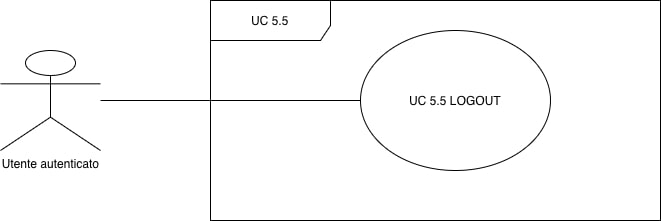
\includegraphics[width=0.8\textwidth]{../UCimg/UC5.5_logout.drawio.jpg}
    \caption{Diagramma del caso d'uso UC-5.5}
    \label{fig:uc5.5}
\end{figure}

\newpage

\section{Requisiti}
\subsection{Classificazione dei requisiti}
Il gruppo ByteMe durante l'analisi dei requisiti e dei casi d'uso ha individuato i requisiti esposti di seguito.
I requisiti sono stati classificati secondo una notazione standardizzata per garantirne la tracciabilità e una chiara comprensione.
Ogni requisito è identificato da un codice univoco che ne esplicita l'importanza e la tipologia.

\subsubsection{Notazione standardizzata dei requisiti}
Il codice identificativo segue il formato:
\[
R[Importanza]-[Tipo]-[Numero]
\]
Dove le voci assumono i seguenti significati:

\begin{description}
    \item[Importanza] \hfill \\
    Indica il grado di priorità del requisito:
    \begin{itemize}
        \item \textbf{O (Obbligatorio):} Requisito esplicitamente richiesto dall'azienda Zucchetti. La sua mancata implementazione implica il fallimento degli obiettivi primari del progetto.
        \item \textbf{D (Desiderabile):} Requisito non strettamente vincolante ma che il gruppo si impegna ad implementare per migliorare il prodotto.
        \item \textbf{OP (Opzionale):} Requisito di priorità minore, la cui implementazione può essere rimandata.
    \end{itemize}
    
    \item[Tipo] \hfill \\
    Indica la natura del requisito:
    \begin{itemize}
        \item \textbf{F (Funzionale):} Descrive le funzionalità e i servizi che il sistema deve fornire.
        \item \textbf{V (Vincolo):} Descrive limitazioni tecnologiche, normative o implementative imposte esternamente.
        \item \textbf{Q (Qualità):} Descrive le caratteristiche qualitative del sistema (es. performance, sicurezza, manutenibilità).
    \end{itemize}
    
    \item[Numero] \hfill \\
    Un numero intero progressivo univoco per tipologia di requisito.
\end{description}

\subsection{Categorie dei Requisiti}
Per una maggiore chiarezza espositiva, i requisiti sono stati suddivisi in tre macro-categorie distinte.

\subsubsection{Requisiti Funzionali}
I requisiti funzionali\textsubscript{G} definiscono i comportamenti specifici del sistema, descrivendo le interazioni tra gli attori e il software.
Rappresentano le funzionalità tangibili che l'utente utilizza per raggiungere i propri obiettivi (es. scrittura del testo, selezione per analisi AI, esportazione documenti). La verifica di tali requisiti determina l'aderenza del prodotto alle funzioni richieste dal capitolato.

\subsubsection{Requisiti Funzionali}
\begin{longtable}{|p{0.2\textwidth}|>{\raggedright\arraybackslash}p{0.5\textwidth}|p{0.2\textwidth}|}
\hline
\textbf{Requisito} & \textbf{Descrizione} & \textbf{Casi d'uso correlati}\\
\hline
\endhead
RO-F-1 & Il sistema deve fornire un editor di testo per l'inserimento e la modifica di caratteri alfanumerici & UC-1.0 \\
\hline
RO-F-2 & L'editor deve compilare la sintassi Markdown & UC-1.1 \\
\hline
RO-F-3 & Deve essere presente un'area di visualizzazione del documento formattato rispetto alla sintassi Markdown & UC-1.1 \\
\hline
RO-F-4 & Il sistema deve permettere all'utente di selezionare porzioni di testo tramite mouse o tastiera & UC-1.2 \\
\hline
RO-F-5 & Il sistema deve permettere all'utente di modificare porzioni di testo selezionate & UC-1.2 \\
\hline
RO-F-6 & Il sistema deve permettere all'utente di copiare una parte del testo & UC-1.3 \\
\hline
RO-F-7 & Il sistema deve permettere all'utente di incollare una parte del testo & UC-1.4 \\
\hline
RO-F-8 & Il sistema deve permettere all'utente di tagliare una parte del testo & UC-1.5 \\
\hline
RO-F-9 & Il sistema deve permettere all'utente di annullare l'ultima modifica effettuata & UC-1.6 \\
\hline
RO-F-10 & Il sistema deve permettere all'utente di ripristinare le modifiche precedentemente cancellate & UC-1.7 \\
\hline
RO-F-11 & Nell'editor è presente una barra degli strumenti (toolbar) per applicare formattazioni Markdown senza scrivere manualmente la sintassi & UC-1.8, UC-1.8.* \\
\hline
RO-F-12 & Il sistema deve permettere l'applicazione del grassetto al testo tramite toolbar & UC-1.8.1 \\
\hline
RO-F-13 & Il sistema deve permettere l'applicazione del corsivo al testo tramite toolbar & UC-1.8.2 \\
\hline
RO-F-14 & Il sistema deve permettere l'applicazione della sottolineatura al testo tramite toolbar & UC-1.8.3 \\
\hline
RO-F-15 & Il sistema deve permettere di creare delle intestazioni e modificare la struttura del testo tramite toolbar & UC-1.8.4 \\
\hline
RO-F-16 & Il sistema deve permettere l'inserimento di liste ed elenchi nel testo tramite toolbar & UC-1.8.5 \\
\hline
RO-F-17 & Il sistema deve permettere l'inserimento di link e riferimenti tramite toolbar & UC-1.8.6 \\
\hline
RO-F-18 & L'utente può applicare più "stili" (es: grassetto, corsivo, sottolineatura) alla stessa sezione di testo & UC-1.8, UC-1.8.* \\
\hline
RO-F-19 & Il sistema deve supportare l'inserimento e la visualizzazione di caratteri Unicode (supporto multilingua) & UC-1.10 \\
\hline
RO-F-20 & Il sistema permette di selezionare del testo & UC-2.0, UC-2.6, UC-2.7, UC-2.7.*, UC-2.9, UC-2.10, UC-2.11 \\
\hline
RO-F-21 & Il sistema permette di avviare la correzione grammaticale & UC-2.6 \\
\hline
RO-F-22 & Il sistema permette di inviare del testo all'AI tramite API REST & UC-2.0, UC-2.6, UC-2.7, UC-2.7.*, UC-2.8, UC-2.9, UC-2.10, UC-2.11 \\
\hline
RO-F-23 & Il sistema può scrivere nell'editor del testo ricevuto dall'AI & UC-2.0, UC-2.2, UC-2.6, UC-2.7, UC-2.7.x, UC-2.8 \\
\hline
RO-F-24 & Il sistema permette all'utente di eliminare il testo generato & UC-2.0, UC-2.2, UC-2.3, UC-2.4, UC-2.5.*, UC-2.6 \\
\hline
RO-F-25 & Il sistema consente all'utente di avviare l'analisi del testo selezionato o dell'intero testo utilizzando il cappello scelto & UC-2.7, UC-2.7.* \\
\hline
RO-F-26 & Il sistema permette l'invio di un prompt per la generazione del testo & UC-2.8 \\
\hline
RO-F-27 & Il sistema permette la modifica del testo generato inserito nell'editor & UC-2.3, UC-2.4, UC-2.5.*, UC-2.8, UC-2.11 \\
\hline
RO-F-28 & Il sistema permette la modifica del prompt da inviare all'AI & UC-2.8, UC-2.9, UC-2.10, UC-2.11 \\
\hline
RO-F-29 & L'utente deve poter accedere alle opzioni AI in ogni momento, per applicare modifiche a tutto il testo & UC-2.0 \\
\hline
RO-F-30 & Ogni sezione IA include opzioni per accettare, eliminare o rigenerare il testo & UC-2.0, UC-2.2, UC-2.3, UC-2.4, UC-2.5.* \\
\hline
RO-F-31 & L'utente deve poter riassumere il testo usando l'IA (selezionato o tutto) & UC-2.3 \\
\hline
RO-F-32 & L'utente deve poter usare l'IA per riscrivere il testo (selezionato o non) & UC-2.4 \\
\hline
RO-F-33 & L'utente deve poter tradurre il testo usando l'IA in: inglese, italiano, tedesco, francese, spagnolo e cinese mandarino & UC-2.5.* \\
\hline
RO-F-34 & Se viene annullata prematuramente la generazione di testo, rimarrà ciò che è già stato generato & UC-2.3, UC-2.4, UC-2.5.* \\
\hline
RO-F-35 & L'utente può caricare/aprire un file dal proprio dispositivo all'interno dell'editor & UC-3.0, UC-3.0.0, UC-3.0.1 \\
\hline
RO-F-36 & Il sistema deve supportare il caricamento tramite dialogo di esplorazione file (file picker) & UC-3.0, UC-3.0.1 \\
\hline
RO-F-37 & Il sistema deve permettere all'utente di rimuovere il file che ha caricato (chiudendo il documento o l'editor) & UC3.0, UC-3.3 \\
\hline
RO-F-38 & Il sistema deve permettere all'utente di annullare l'operazione di caricamento file & UC-3.0 \\
\hline
RO-F-39 & Il sistema notifica l'errore se non riesce a caricare il file & UC-3.1, UC-3.2\\
\hline
RD-F-1 & Il sistema deve supportare l'uso di scorciatoie da tastiera per le operazioni di formattazione & UC-1.8.* \\
\hline
RD-F-2 & Il sistema deve permettere di cambiare modalità di visualizzazione (Solo Editor, Solo Anteprima, Split View) & UC-1.9 \\
\hline
RD-F-3 & Il sistema deve supportare il caricamento tramite drag-and-drop (trascinamento file nell'area dell'editor) & UC-3.0, UC-3.0.0 \\
\hline
RD-F-4 & L'utente deve visualizzare un menù di opzioni per le azioni da fare sul file (carica, nuovo, stampa, chiudi) & UC-1.0, UC-3.0, UC-3.3 \\
\hline
RD-F-5 & Se sono presenti modifiche non salvate nell'editor, il sistema chiede conferma all'utente prima di caricare un nuovo file, permettendo di annullare l'operazione, per salvare il testo presente, o sovrascrivere il contenuto senza salvarlo & UC-3.0 \\
\hline
ROP-F-1 & L'utente può ricercare parole nel testo attraverso l'editor & UC-1.10 \\
\hline
ROP-F-2 & AI crea una riga separatrice tra il testo generato e quello utente ('---') & UC-2.0, UC-2.2, UC-2.3, UC-2.4, UC-2.5.* \\
\hline
ROP-F-3 & La sezione viene colorata in base al tipo di operazione che viene fatta & UC-2.2 \\
\hline
ROP-F-4 & Il sistema offre esempi per la richiesta di generazione di testo a partire da un estratto & UC-2.8 \\
\hline
ROP-F-5 & Il sistema inserisce un grafico generato scelto tra diversi tipi disponibili all'utente & UC-2.9 \\
\hline
ROP-F-6 & Il sistema inserisce una tabella generata & UC-2.9 \\
\hline
ROP-F-7 & Il sistema inserisce una mappa concettuale generata & UC-2.10 \\
\hline
ROP-F-8 & Il sistema inserisce una formula matematica generata & UC-2.11 \\
\hline
ROP-F-9 & Il sistema permette all'utente di avviare la generazione di testo tramite un comando rapido /genera seguito da un prompt testuale & UC-2.8 \\
\hline
ROP-F-10 & Il sistema deve permettere all'utente di inserire le proprie credenziali (username e password) per il login & UC-5.0 \\
\hline
ROP-F-11 & Se le credenziali sono errate il sistema deve non far autenticare l'utente & UC-5.0 \\
\hline
ROP-F-12 & Il sistema deve permettere all'utente di potersi registrare tramite uno username e una password & UC-5.1 \\
\hline
ROP-F-13 & Il sistema deve impedire la registrazione in caso ci sia uno username uguale nel database & UC-5.1 \\
\hline
ROP-F-14 & Il sistema deve salvare nel database le password criptate in fase di registrazione & UC-5.1 \\
\hline
ROP-F-15 & Il sistema deve permettere ad un utente autenticato di poter eliminare il proprio account & UC-5.2 \\
\hline
ROP-F-16 & Il sistema in caso di eliminazione account deve eliminare i dati dal database & UC-5.2 \\
\hline
ROP-F-17 & Le operazioni di eliminazione dell'account devono richiedere una conferma esplicita da parte dell'utente & UC-5.2 \\
\hline
ROP-F-18 & Il sistema deve terminare la sessione nel caso un account venga eliminato & UC-5.2 \\
\hline
ROP-F-19 & Il sistema deve permettere ad un utente di vedere i file che ha salvato & UC-5.3 \\
\hline
ROP-F-20 & Il sistema deve permettere ad un utente autenticato di selezionare un file dall'elenco e aprirlo & UC-5.3 \\
\hline
ROP-F-21 & Il sistema deve consentire all'utente di annullare l'operazione di apertura senza recuperare alcun file dal database & UC-5.3 \\
\hline
ROP-F-22 & Il sistema deve permettere all'utente l'apertura di un file salvato e visibile all'utente & UC-5.3 \\
\hline
ROP-F-23 & Il sistema deve permettere il salvataggio di un file in un sistema di persistenza non locale & UC-5.4 \\
\hline
ROP-F-24 & Il sistema deve associare ogni file al suo creatore & UC-5.4 \\
\hline
ROP-F-25 & L'utente può effettuare il logout in ogni momento e terminare la propria sessione & UC-5.5 \\
\hline

\addlinespace[1em]
\caption{Tabella dei requisiti funzionali}
\end{longtable}

\newpage
\subsubsection{Requisiti di Vincolo}
I requisiti di vincolo\textsubscript{G} rappresentano le limitazioni entro le quali il progetto deve essere sviluppato. A differenza dei requisiti funzionali, questi non derivano da scelte progettuali del team, ma sono imposizioni esterne dettate dal committente, da normative o da limiti tecnologici.
Questi comprendono i vincoli tecnologici, architetturali e organizzativi.

% tabella per i requisiti non funzionali di vincolo
\begin{longtable}{|p{0.2\textwidth}|>{\raggedright\arraybackslash}p{0.5\textwidth}|p{0.2\textwidth}|}
\hline
\textbf{Requisito} & \textbf{Descrizione} & \textbf{Casi d'uso correlati}\\
\hline

RO-V-1 & L'applicazione deve essere accessibile via browser e necessita di connessione internet & UC-1.0 \\
\hline
RO-V-2 & Il sistema deve supportare nativamente la codifica dei caratteri Unicode (UTF-8) per garantire la leggibilità di testi multilingua & UC-1.10 \\
\hline
RO-V-3 & Il formato di input e storage del testo deve essere Markdown & UC-1.0, UC-1.1 \\
\hline
RO-V-4 & AI deve sapere cosa è stato selezionato e incorporare le modifiche selezionate solo per quella parte di testo & UC-2.0 \\
\hline
RO-V-5 & AI deve mantenere il contesto di tutto il testo scritto quando viene chiamato, anche se sta agendo solo su una parte & UC-2.0 \\
\hline
RO-V-6 & Il testo generato dall'AI viene creato in una nuova sezione in fondo al testo & UC-2.0, UC-2.2 \\
\hline
RO-V-7 & Le sezioni che includono un riassunto diranno anche quali righe ha riassunto & UC-2.3, UC-2.4, UC-2.5.* \\
\hline
RO-V-8 & L'AI deve avere istruzioni sufficienti affinché il testo riscritto sia corretto grammaticalmente, sintatticamente e semanticamente e deve riflettere la richiesta dell'utente & UC-2.4 \\
\hline
RO-V-9 & Le sezioni create per la traduzione di un testo specificheranno la lingua di partenza e di fine & UC-2.5.* \\
\hline
RO-V-10 & Se il testo è già nella lingua da tradurre, l'AI genera avvisa l'utente e interrompe l'operazione & UC-2.5.* \\
\hline
RO-V-11 & AI deve avere delle istruzioni ottimizzate per la traduzione nella lingua selezionata & UC-2.5.* \\
\hline
RO-V-12 & Il sistema espone la sua limitazione nell'eseguire un'azione richiesta se i dati inviati non rispettano i limiti dell'AI & UC-2.9, UC-2.10, UC-2.11 \\
\hline
RO-V-13 & Il caricamento e la lettura del file devono avvenire localmente tramite le API del browser (es. File API), senza inviare il contenuto a un server & UC-3.* \\
\hline
RD-V-1 & Il sistema deve supportare l'importazione dei formati di file più comuni: .md, .txt, .markdown & UC-3.0, UC-3.2 \\
\hline
ROP-V-1 & La password inserita dall'utente deve essere minimo 8 caratteri & UC-5.1 \\
\hline
ROP-V-2 & La password inserita dall'utente deve contenere almeno un carattere speciale & UC-5.1 \\
\hline
ROP-V-3 & L'accesso ai file salvati nel database deve essere consentito solo ad utenti autenticati & UC-5.3 \\
\hline
ROP-V-4 & Il sistema deve impedire il salvataggio di file nel database da parte di utenti non autenticati & UC-5.4 \\
\hline
\addlinespace[1em]
\caption{Tabella dei requisiti di vincolo}
\end{longtable}


\newpage
\subsubsection{Requisiti di Qualità}
I requisiti di qualità\textsubscript{G} specificano le caratteristiche intrinseche del software. Non descrivono nuove funzioni, ma stabiliscono \textit{come} il sistema deve erogare quelle esistenti. 
% tabella per i requisiti non funzionali di qualità
\begin{longtable}{|p{0.2\textwidth}|>{\raggedright\arraybackslash}p{0.5\textwidth}|p{0.2\textwidth}|}
\hline
\textbf{Requisito} & \textbf{Descrizione} & \textbf{Casi d'uso correlati}\\
\hline

RO-Q-1 & Il sistema deve compilare il testo markdown in un breve lasso di tempo & UC-1.0, UC-1.1 \\
\hline
RO-Q-2 & Il sistema deve fornire messaggi di errore chiari se l'editor non risponde o se l'anteprima fallisce & UC-1.0, UC-1.1 \\
\hline
RO-Q-3 & L'aggiornamento dell'anteprima compilata deve avvenire in tempi brevi dopo la richiesta di compilazione & UC-1.0, UC-1.1 \\
\hline
RO-Q-4 & L'LLM deve rispondere sempre in tempi brevi, o restituire errore & UC-2.* \\
\hline
RO-Q-5 & Le opzioni AI devono apparire velocemente & UC-2.0 \\
\hline
RO-Q-6 & Le opzioni non devono sparire in maniera poco intuitiva muovendo il mouse & UC-2.0 \\
\hline
RO-Q-7 & Il testo creato si comporta come qualunque altro testo aggiunto dall'IA: facilmente riconoscibile e sempre modificabile dall'utente & UC-2.3, UC-2.4, UC-2.5.*, UC-2.8 \\
\hline
RO-Q-8 & Il sistema mostra un messaggio in caso di errore durante la generazione di contenuto & UC-2.3, UC-2.4, UC-2.5.*, UC-2.6, UC-2.7, UC-2.7.*, UC-2.8, UC-2.9, UC-2.10, UC-2.11 \\
\hline
RO-Q-9 & Il sistema deve fornire un feedback visivo immediato all'utente (messaggio di errore o di successo) al termine del tentativo di caricamento file & UC-3.0, UC-3.1, UC-3.2 \\
\hline
RO-Q-10 & Il sistema deve validare il formato del file caricato e impedire il caricamento di formati non supportati & UC-3.1 \\
\hline
RO-Q-11 & Il sistema deve validare le dimensioni del file caricato e impedire il caricamento di file che superano una dimensione massima & UC-3.2 \\
\hline
RO-Q-12 & Il sistema deve impedire il caricamento di file corrotti & UC-3.0, UC-3.1\\
\hline
RO-Q-13 & La dimensione massima consentita per il caricamento di un file deve essere limitata a una soglia definita e ragionevole & UC-3.0, UC-3.2 \\
\hline
RD-Q-1 & I messaggi di errore (per formato errato, file troppo grande o corrotto) devono essere esplicativi e suggerire all'utente come procedere & UC-3.0, UC-3.2, UC-3.3 \\
\hline
RD-Q-2 & L'operazione di caricamento e rendering di un file di dimensioni supportate deve completarsi in meno di 3 secondi & UC-3.0, UC-3.0.0, UC-3.0.1 \\
\hline
RD-Q-3 & Il parsing del contenuto del file deve essere robusto, garantendo che caratteri non validi non causino il crash dell'applicazione & UC-3.* \\
\hline
ROP-Q-1 & Il sistema deve mostrare un messaggio di errore non specifico nel caso di fallimento del login & UC-5.0 \\
\hline
ROP-Q-2 & Il sistema deve avvisare l'utente che lo username è già stato usato & UC-5.1 \\
\hline
ROP-Q-3 & Il sistema propone all'utente di effettuare il login o scegliere un nuovo username & UC-5.1 \\
\hline
ROP-Q-4 & Il sistema mostra i file salvati in ordine cronologico & UC-5.3 \\
\hline
ROP-Q-5 & Il sistema deve notificare all'utente il fallimento del salvataggio & UC-5.4 \\
\hline
\addlinespace[1em]
\caption{Tabella dei requisiti di qualità}
\end{longtable}

\newpage

\section{Riepilogo}
\begin{table}[H]
\centering
\begin{tabular}{|p{0.2\textwidth}|>{\raggedright\arraybackslash}p{0.1\textwidth}|p{0.1\textwidth}|p{0.1\textwidth}|p{0.1\textwidth}|}
\hline
\textbf{Tipologia} & \textbf{O} & \textbf{D} & \textbf{OP} & \textbf{Totale}\\
\hline
Funzionali & 39 & 5 & 25 & 69 \\
\hline
Vincolo & 13 & 1 & 4 & 18 \\
\hline
Qualità & 13 & 3 & 5 & 21 \\
\hline
\textbf{Totale} & 65 & 9 & 34 & 108\\
\hline
\end{tabular}
\caption{Riepilogo dei requisiti}
\end{table}


\end{document}
